\documentclass{article}

% 导入宏包
\usepackage{fancyhdr}
\usepackage{ctex}
\usepackage{listings}
\usepackage{graphicx}
\usepackage[a4paper, body={18cm,22cm}]{geometry}
\usepackage{amsmath,amsthm,amssymb,amstext,wasysym,enumerate,graphicx}
\usepackage{float,abstract,booktabs,indentfirst,amsmath}
\usepackage{array}
\usepackage{multirow}
\usepackage{multicol}
\usepackage{url}
\usepackage{diagbox}
\usepackage{enumitem}
\usepackage{xcolor}
\usepackage{makecell}
\usepackage{tikz}
\usepackage{tcolorbox}
\usetikzlibrary{positioning, arrows.meta}
\usepackage[bookmarks=true, colorlinks, citecolor=blue, linkcolor=black]{hyperref}


% 设置段落
\renewcommand\arraystretch{1.4}
\setlength{\parindent}{2em}
\setCJKmonofont{黑体}

% 设置高亮文字
\newtcbox{\mybox}[1][red]
{on line, arc = 0pt, outer arc = 0pt,
	colback = #1!10!white, colframe = #1!50!black,
	boxsep = 0pt, left = 1pt, right = 1pt, top = 2pt, bottom = 2pt,
	boxrule = 0pt, bottomrule = 1pt, toprule = 1pt}

% 配置代码显示
\lstset{
	xleftmargin = 3em,
	xrightmargin = 3em,
	aboveskip = 1em,
	backgroundcolor = \color{white},
	basicstyle = \small\ttfamily,
	rulesepcolor = \color{gray},
	breaklines = true,
	numbers = left,
	numberstyle = \small,
	numbersep = -14pt,
	keywordstyle = \color{purple}\bfseries,
	commentstyle = \color{green!60!black}, % 修改注释颜色
	stringstyle = \color{red!60!green!90!blue!90},
	morekeywords = {ASSERT, int64_t, uint32_t},
	moreemph = {ASSERT, NULL},
	emphstyle = \color{red}\bfseries,
	moreemph = [2]{int64\_t, uint32\_t, tid\_t, uint8\_t, int16\_t, uint16\_t, int32\_t, size\_t, bool},
	emphstyle = [2]\color{purple}\bfseries,
	frame = shadowbox,
	showspaces = false,
	columns = fixed
	morecomment = [l][\color{green!60!black}]{+}, % 设置以+开头的代码行为绿色
}

%--------------------页眉--------------------%

\pagestyle{fancy}
\fancyhead[L]{}
\fancyhead[R]{}
\fancyhead[C]{华东师范大学软件工程学院实验报告}
\fancyfoot[C]{-\thepage-}
\renewcommand{\headrulewidth}{1.5pt}

%--------------------标题--------------------%

\begin{document}
	\begin{center}
		{\Large{\textbf{\heiti 华东师范大学软件工程学院实验报告}}}
		\begin{table}[htb]
			\flushleft
			\begin{tabular}{p{0.4\linewidth}p{0.27\linewidth}p{0.28\linewidth}}\\
				\textbf{实验课程}:数据库系统及其应用实践  & \textbf{年级}:2023级       & \textbf{实验成绩}:  \\
				\textbf{实验名称}:Lab-04 & \textbf{姓名}:顾翌炜         &                 \\
				\textbf{实验编号}:Lab-04     & \textbf{学号}:10235101527 & \textbf{实验日期}:2025/04/24  \\
				\textbf{指导教师}:姚俊杰     & \textbf{组号}:01            & \textbf{实验时间}:2课时  \\ 
			\end{tabular}
		\end{table}
	\end{center}
	\rule{\textwidth}{2pt}
	
	% 重新定义目录环境为两列
	\makeatletter
	\renewcommand{\tableofcontents}{%
		\begin{multicols}{2}[\section*{\contentsname}]%
			\@starttoc{toc}%
		\end{multicols}%
	}
	\makeatother
	
	% 生成目录
	\tableofcontents
	
	\clearpage
	
	\section{实验目标}
	
	通过开源项目DB-GPT和外部大模型,尝试利用大模型进行数据管理和数据库交互,完成作业。
	
	\section{实验要求}
	
	\begin{enumerate}[noitemsep, label={{\arabic*})}]
		\item 实验相关文件中包括了实验1-SQL编写练习中使用的两个数据库的sqlite版本。可以直接使用两个数据库测试LLMs的sql编写和数据处理能力;也可以自选感兴趣的其他数据库场景尝试(可以通过kaggle网站找找自己感兴趣的领域数据集,https://www.kaggle.com/)。【使用chat data模块功能】
		
		\item 实验报告中需要记录:项目搭建和运行的过程、测试通过LLMs进行数据库检索的效果(至少10个场景问题的尝试,复杂,有趣和具有连续多轮对话的应用问题最好)
	\end{enumerate}\textbf{}
	
	\subsection{实验环境}
	
	\begin{enumerate}[noitemsep, label={{\arabic*})}]
		\item Anaconda(用于环境管理)
		\item UV(用于依赖安装和项目运行)
		\item Git(用于代码克隆)
		\item 阿里云模型服务(灵积平台)
	\end{enumerate}\textbf{}
	
	\section{实验过程记录}
	
	\subsection{环境配置}
	
	由于我之前已经下载过anaconda,所以此处不展示下载过程,直接使用
	
	打开如图所示的Anaconda Powershell Prompt
	
	\begin{figure}[H]
		\centering
		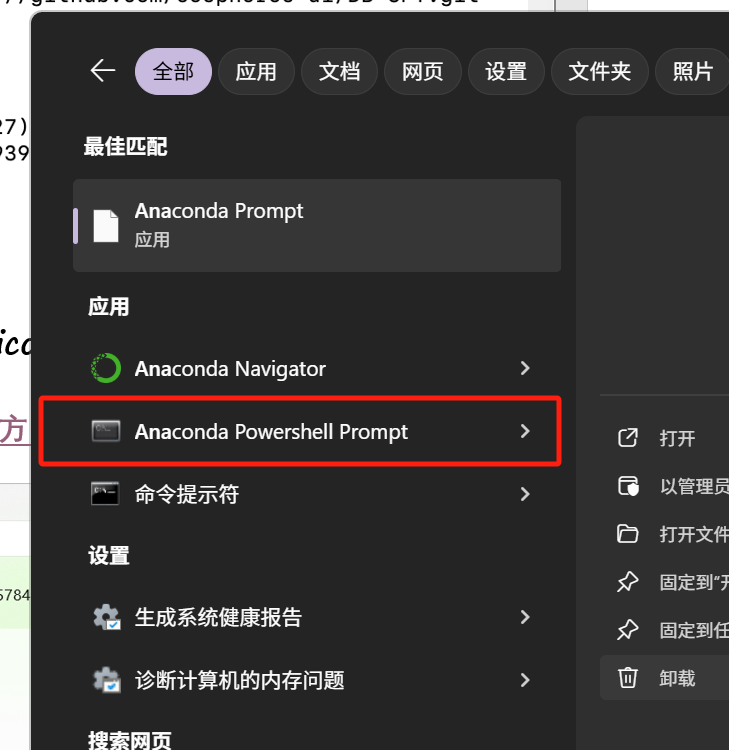
\includegraphics[width=9cm]{./images/1.anaconda powershell.png}
		\caption{anaconda powershell}
	\end{figure}
	
	利用以下指令创建虚拟环境
	
	\begin{lstlisting}[language=bash, title=创建虚拟环境, tabsize=4]
	conda create -n dbgpt_env python=3.10
	\end{lstlisting}
	
	\begin{figure}[H]
		\centering
		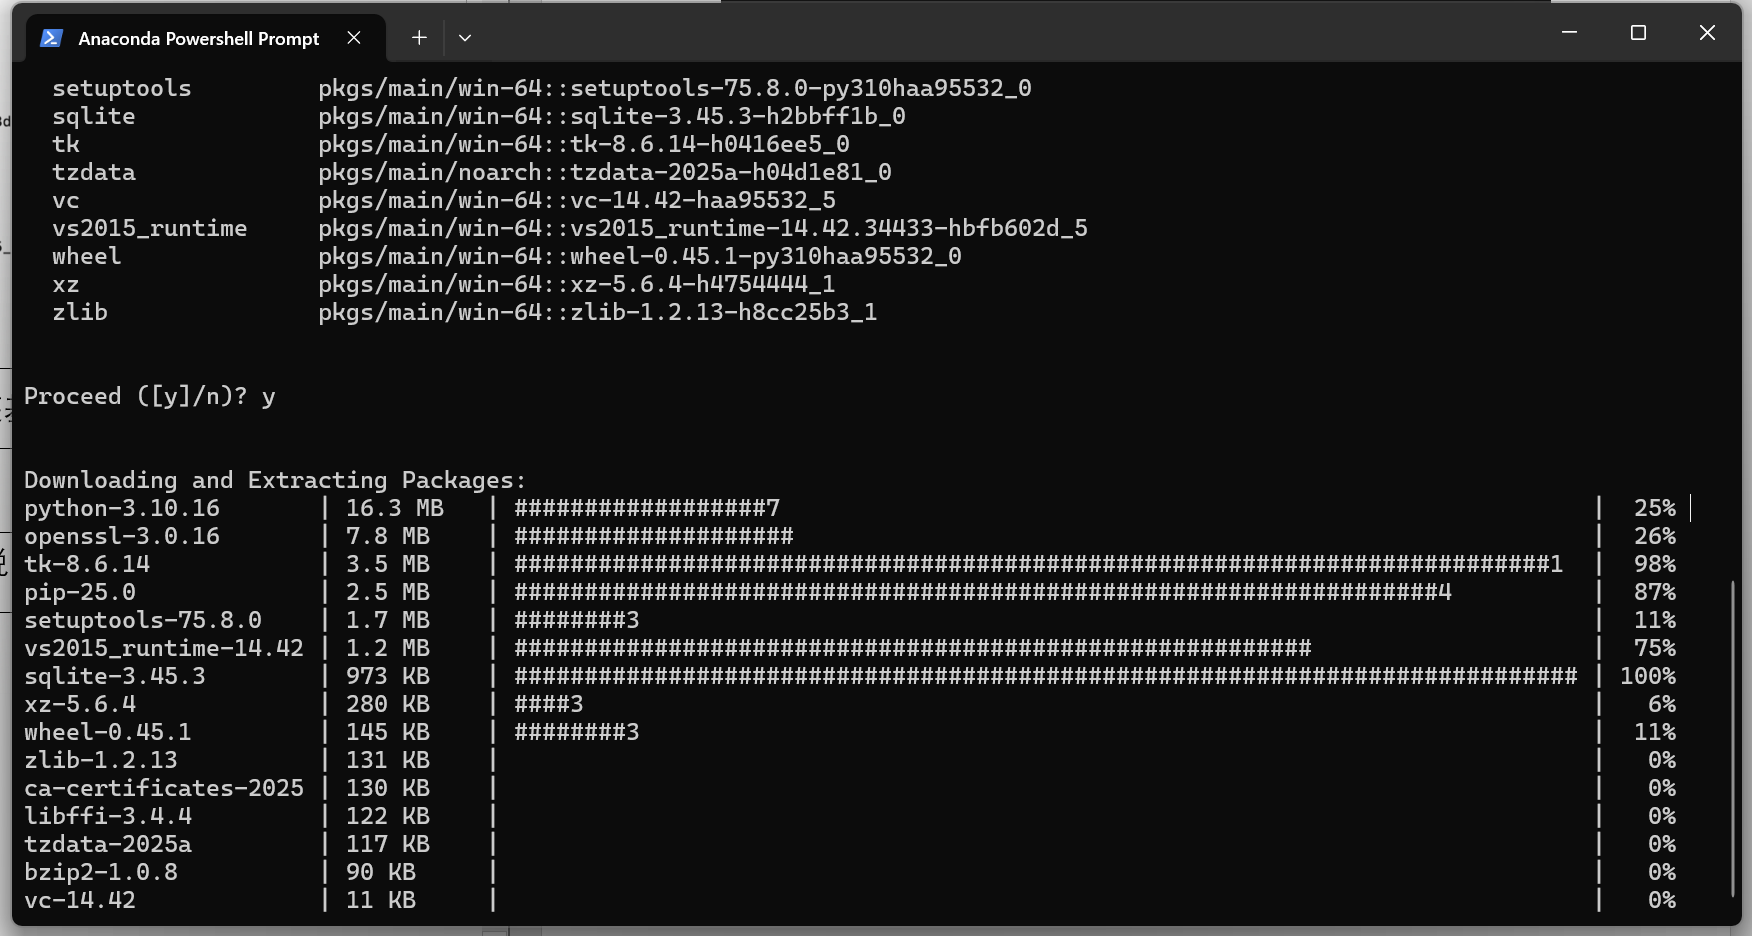
\includegraphics[width=12cm]{./images/2.创建虚拟环境.png}
		\caption{创建虚拟环境}
	\end{figure}
	
	等待下载完成
	
	\begin{figure}[H]
		\centering
		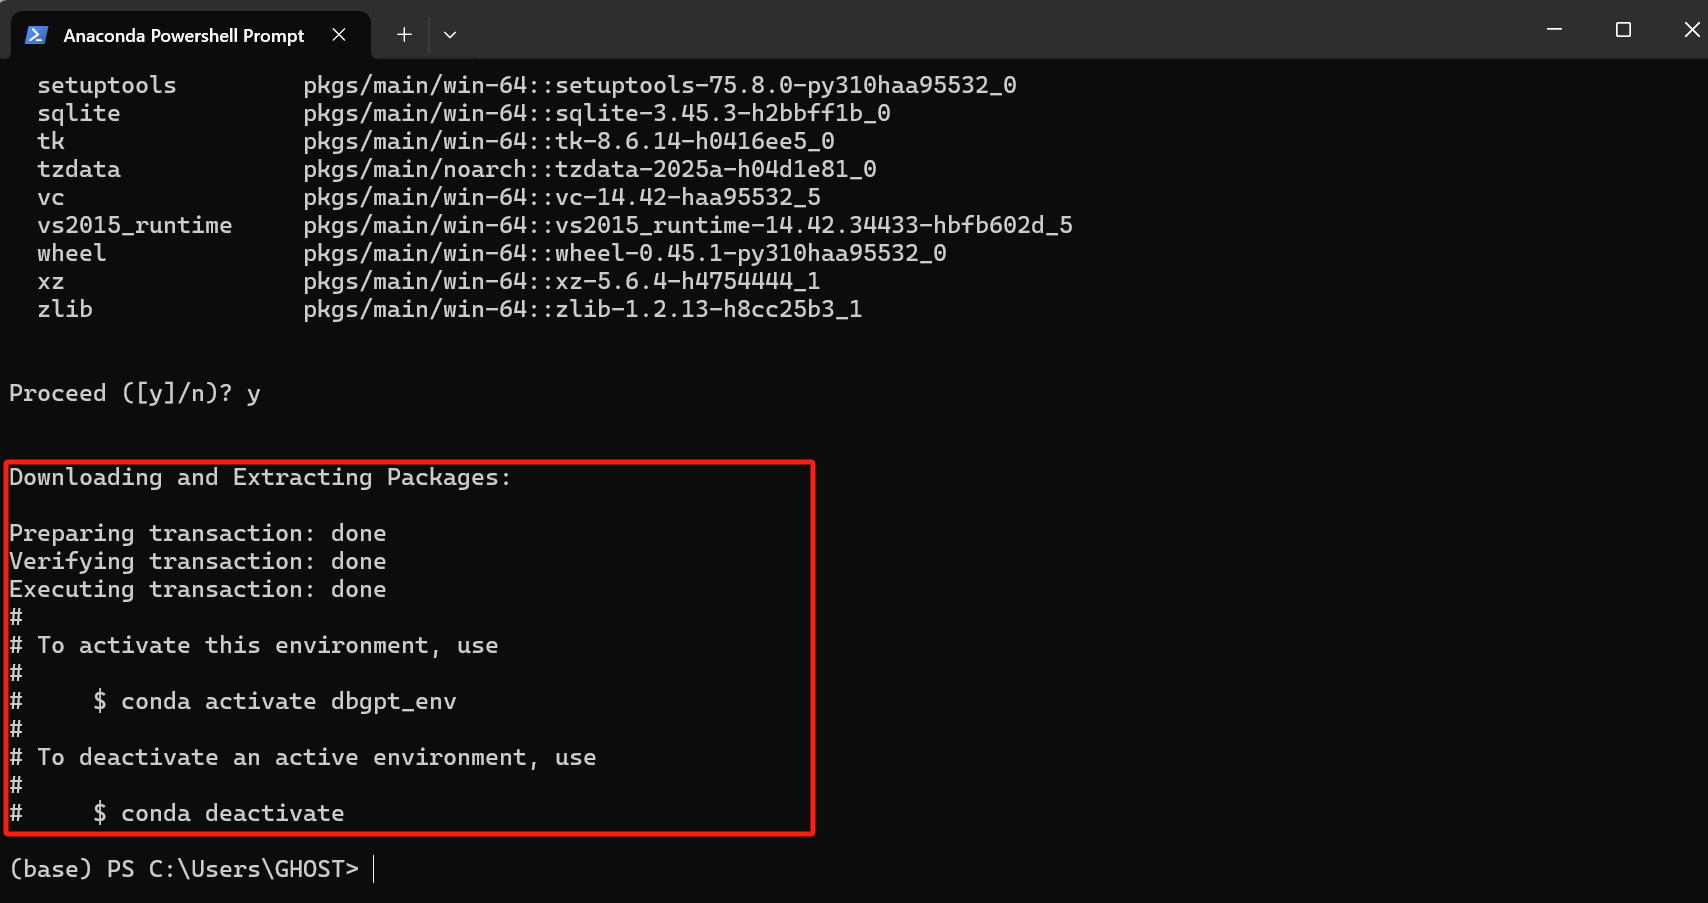
\includegraphics[width=11cm]{./images/3.虚拟环境安装完成.png}
		\caption{虚拟环境安装完成}
	\end{figure}
	
	利用下面的指令来激活虚拟环境
	
	\begin{lstlisting}[language=bash, title=激活虚拟环境, tabsize=4]
	conda activate dbgpt_env
	\end{lstlisting}
	
	\begin{figure}[H]
		\centering
		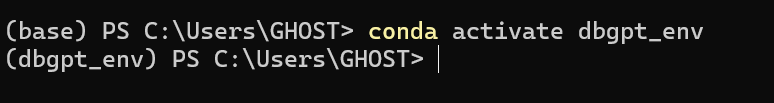
\includegraphics[width=11cm]{./images/4.激活虚拟环境.png}
		\caption{激活虚拟环境}
	\end{figure}
	
	\subsection{uv安装}
	
	为了提升速度建议使用国内的镜像,我执行的命令是:
	
	\begin{lstlisting}[language=bash, title=uv安装, tabsize=4]
	powershell -ExecutionPolicy ByPass -c "irm https://astral.sh/uv/install.ps1 | iex"
	\end{lstlisting}
	
	\begin{figure}[H]
		\centering
		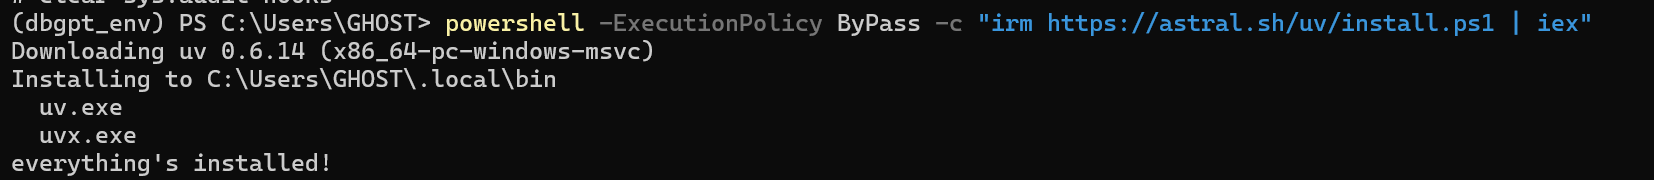
\includegraphics[width=13cm]{./images/5.安装uv.png}
		\caption{安装uv}
	\end{figure}
	
	使用以下命令测试是否uv安装成功:
	
	\begin{lstlisting}[language=bash, title=uv安装, tabsize=4]
		uv --version
	\end{lstlisting}
	
	得到结果:uv 0.6.14 (a4cec56dc 2025-04-09)
	
	\begin{figure}[H]
		\centering
		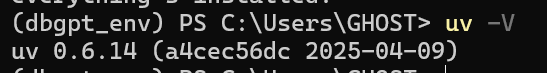
\includegraphics[width=11cm]{./images/6.检查uv.png}
		\caption{检查uv}
	\end{figure}
	
	安装uv完成,继续下一步实验
	
	\subsection{下载源代码}
	
	首先使用git clone来克隆代码
	
	\begin{figure}[H]
		\centering
		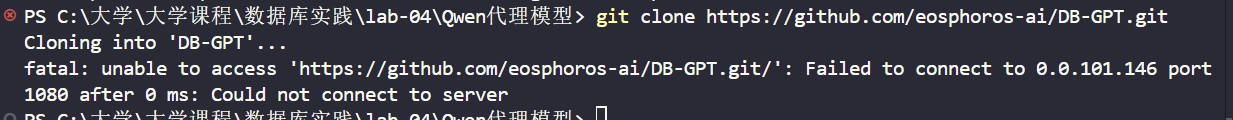
\includegraphics[width=11cm]{./images/7.git clone.png}
		\caption{git clone}
	\end{figure}
	
	查看vpn的端口号,发现端口号未绑定,所以连接不上github
	
	\begin{figure}[H]
		\centering
		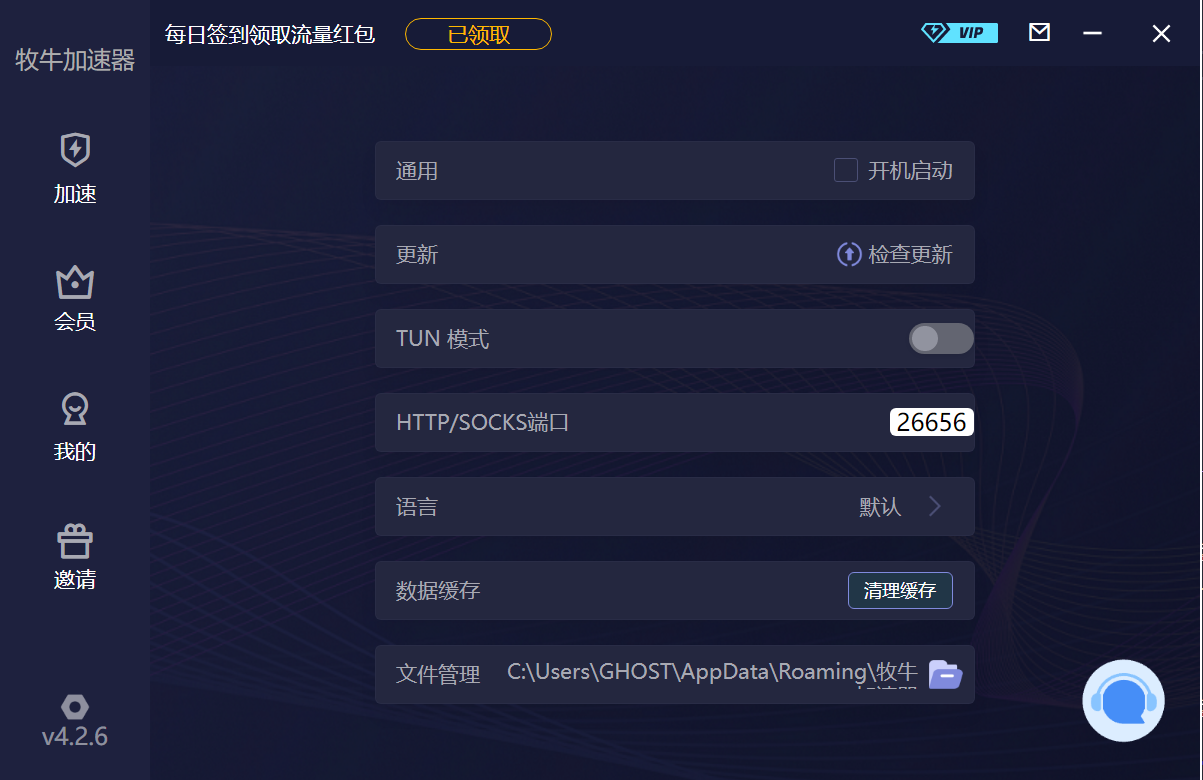
\includegraphics[width=11cm]{./images/8.检查vpn端口号.png}
		\caption{检查vpn端口号}
	\end{figure}
	
	利用以下代码设置代理端口
	
	\begin{lstlisting}[language=bash, title=uv安装, tabsize=4]
		git config --global http.proxy socks5://127.0.0.1:26656
		git config --global https.proxy socks5://127.0.0.1:26656
	\end{lstlisting}
	
	设置好代理端口以后,重新clone
	
	\begin{figure}[H]
		\centering
		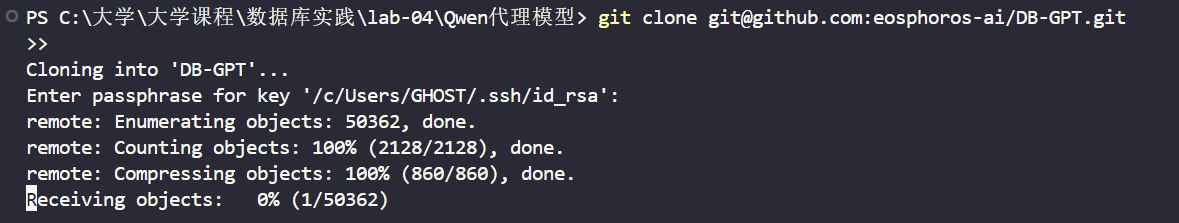
\includegraphics[width=11cm]{./images/9.重新clone.png}
		\caption{重新clone}
	\end{figure}
	
	克隆结束,打开DB-GPT文件夹,可以看到:
	
	\begin{figure}[H]
		\centering
		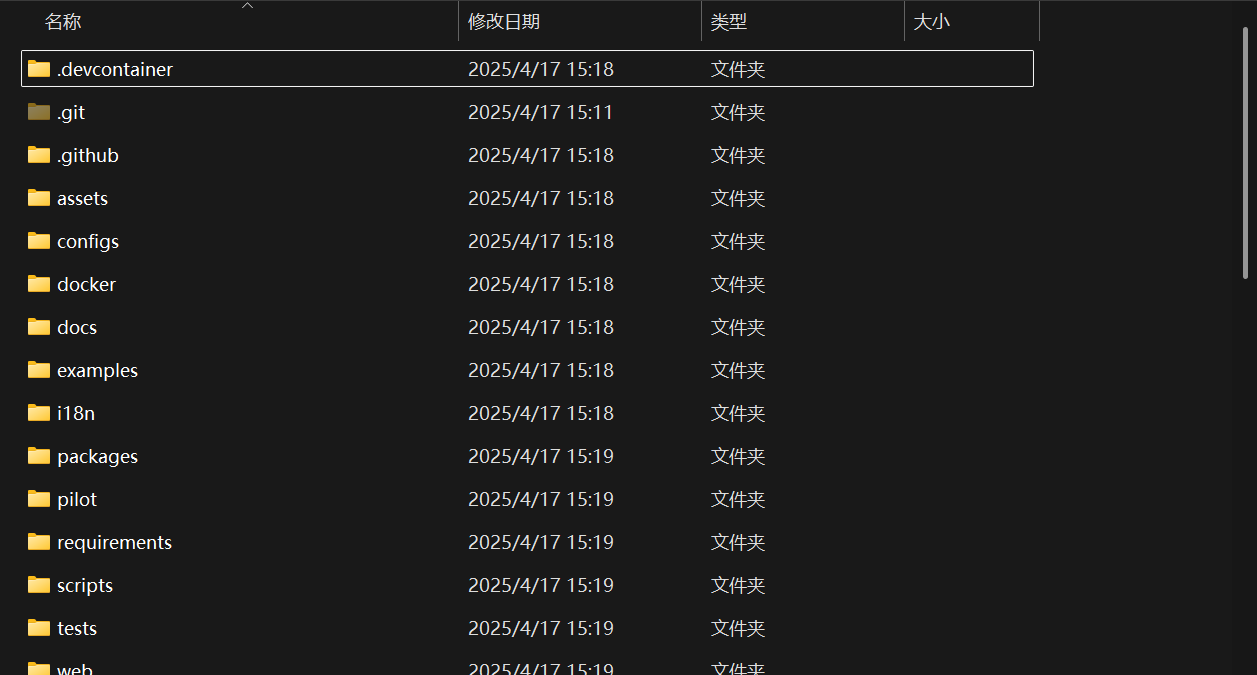
\includegraphics[width=11cm]{./images/10.DB-GPT文件夹.png}
		\caption{DB-GPT文件夹}
	\end{figure}
	
	用以下命令进入到DB-GPT文件夹:
	
	\begin{lstlisting}[language=bash, title=uv安装, tabsize=4]
		cd DB-GPT
	\end{lstlisting}
	
	\subsection{依赖安装}
	
	需要选择安装全量依赖:
	
	\begin{lstlisting}[language=bash, title=uv安装, tabsize=4]
		uv sync --all-packages --frozen --extra "base" --extra "proxy_openai" --extra "hf" --extra "llama_cpp" --extra "rag" --extra "storage_chromadb" --extra "dbgpts" --extra "quant_bnb"
	\end{lstlisting}
	
	\begin{figure}[H]
		\centering
		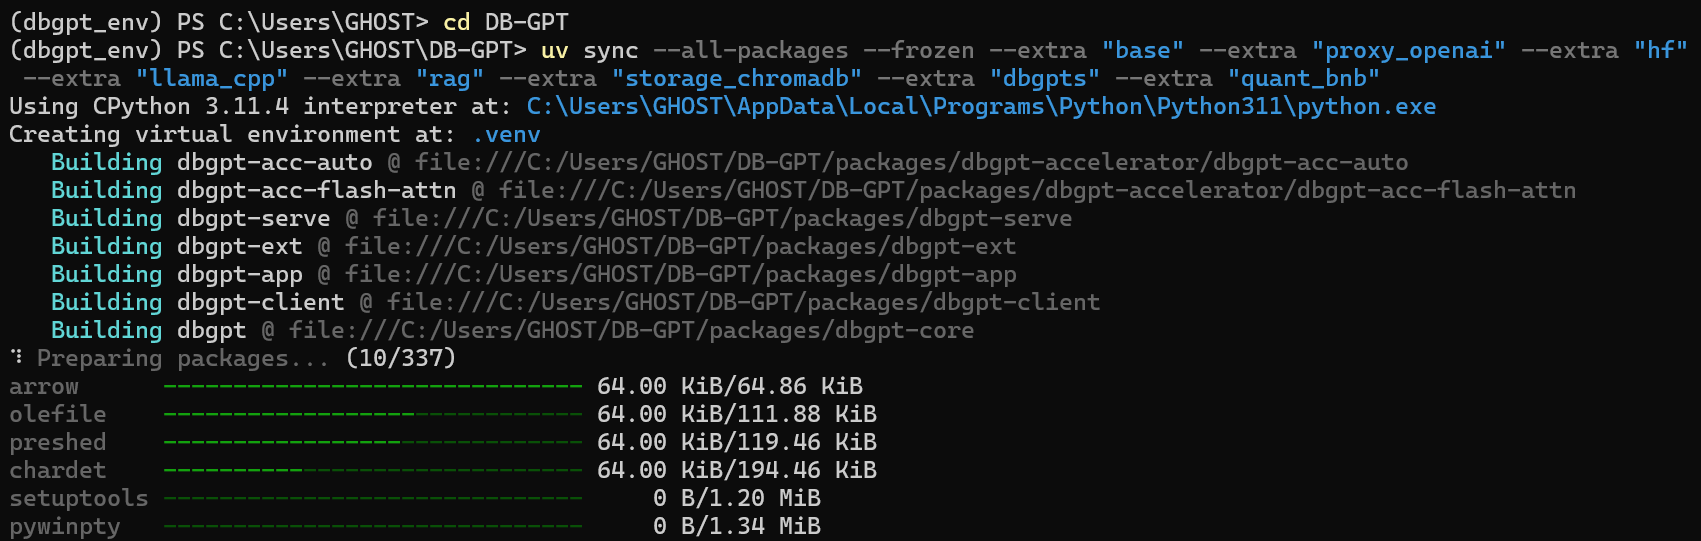
\includegraphics[width=13cm]{./images/11.依赖安装.png}
		\caption{依赖安装}
	\end{figure}
	
	接下来,耐心等待环境安装结束即可
	
	\subsection{注册阿里云账户号并申请api}
	
	注册阿里云账号,选择模型服务灵积
	
	\begin{figure}[H]
		\centering
		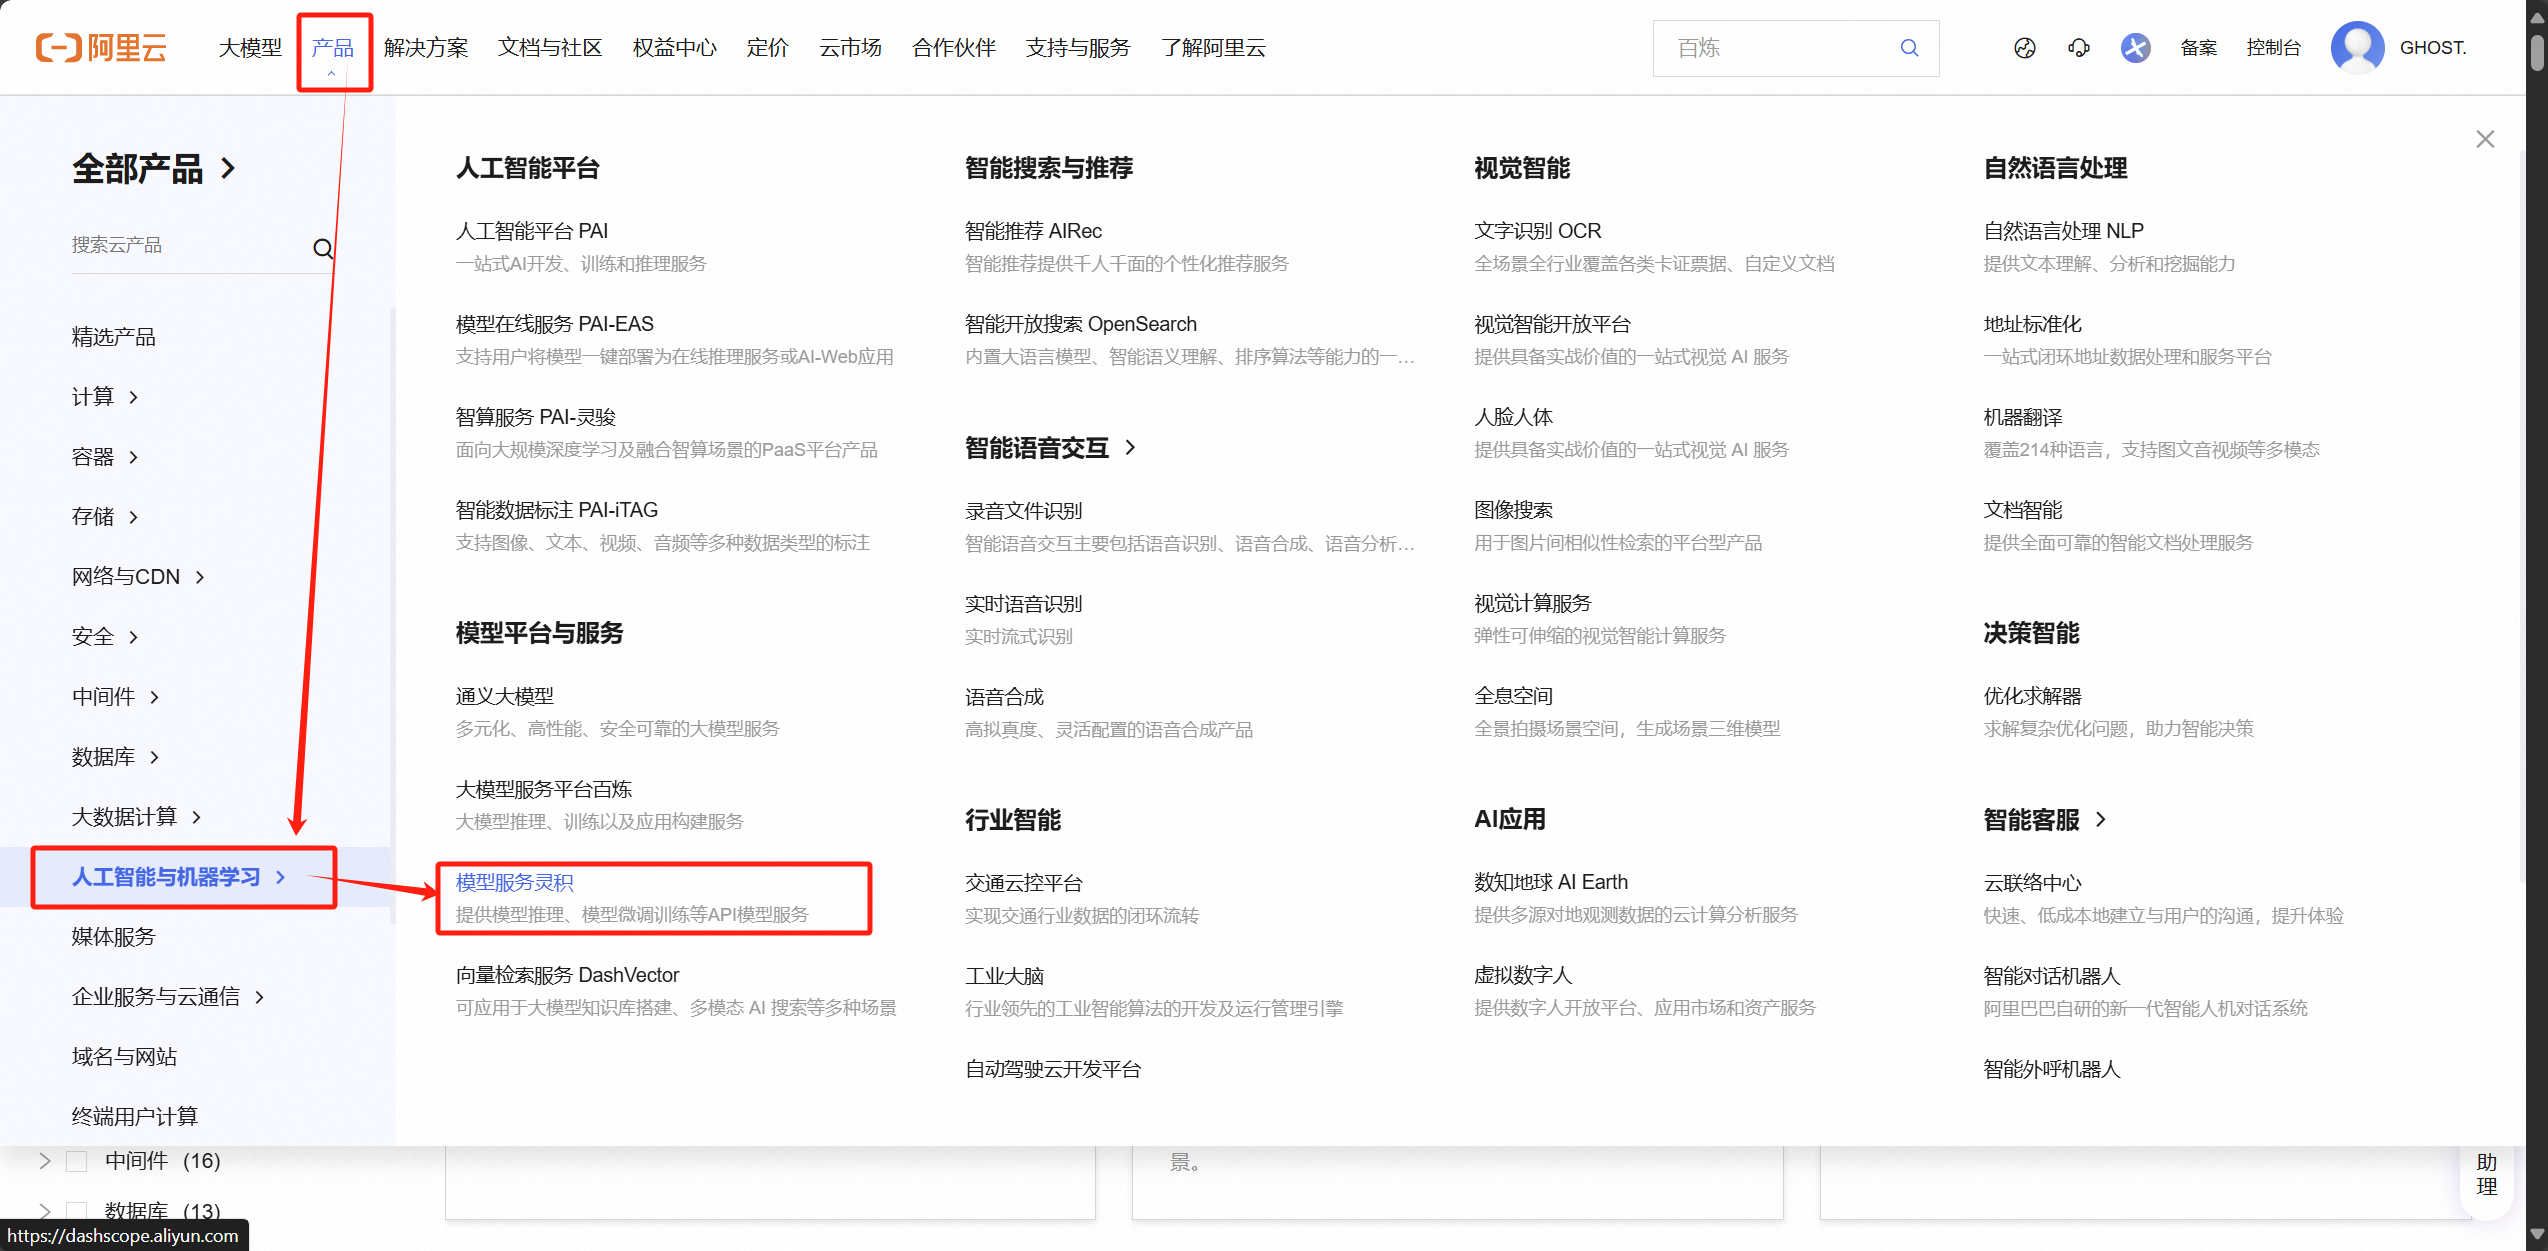
\includegraphics[width=13cm]{./images/12.模型服务灵积.png}
		\caption{模型服务灵积}
	\end{figure}
	
	在官网上,按照教程创建api
	
	\begin{figure}[H]
		\centering
		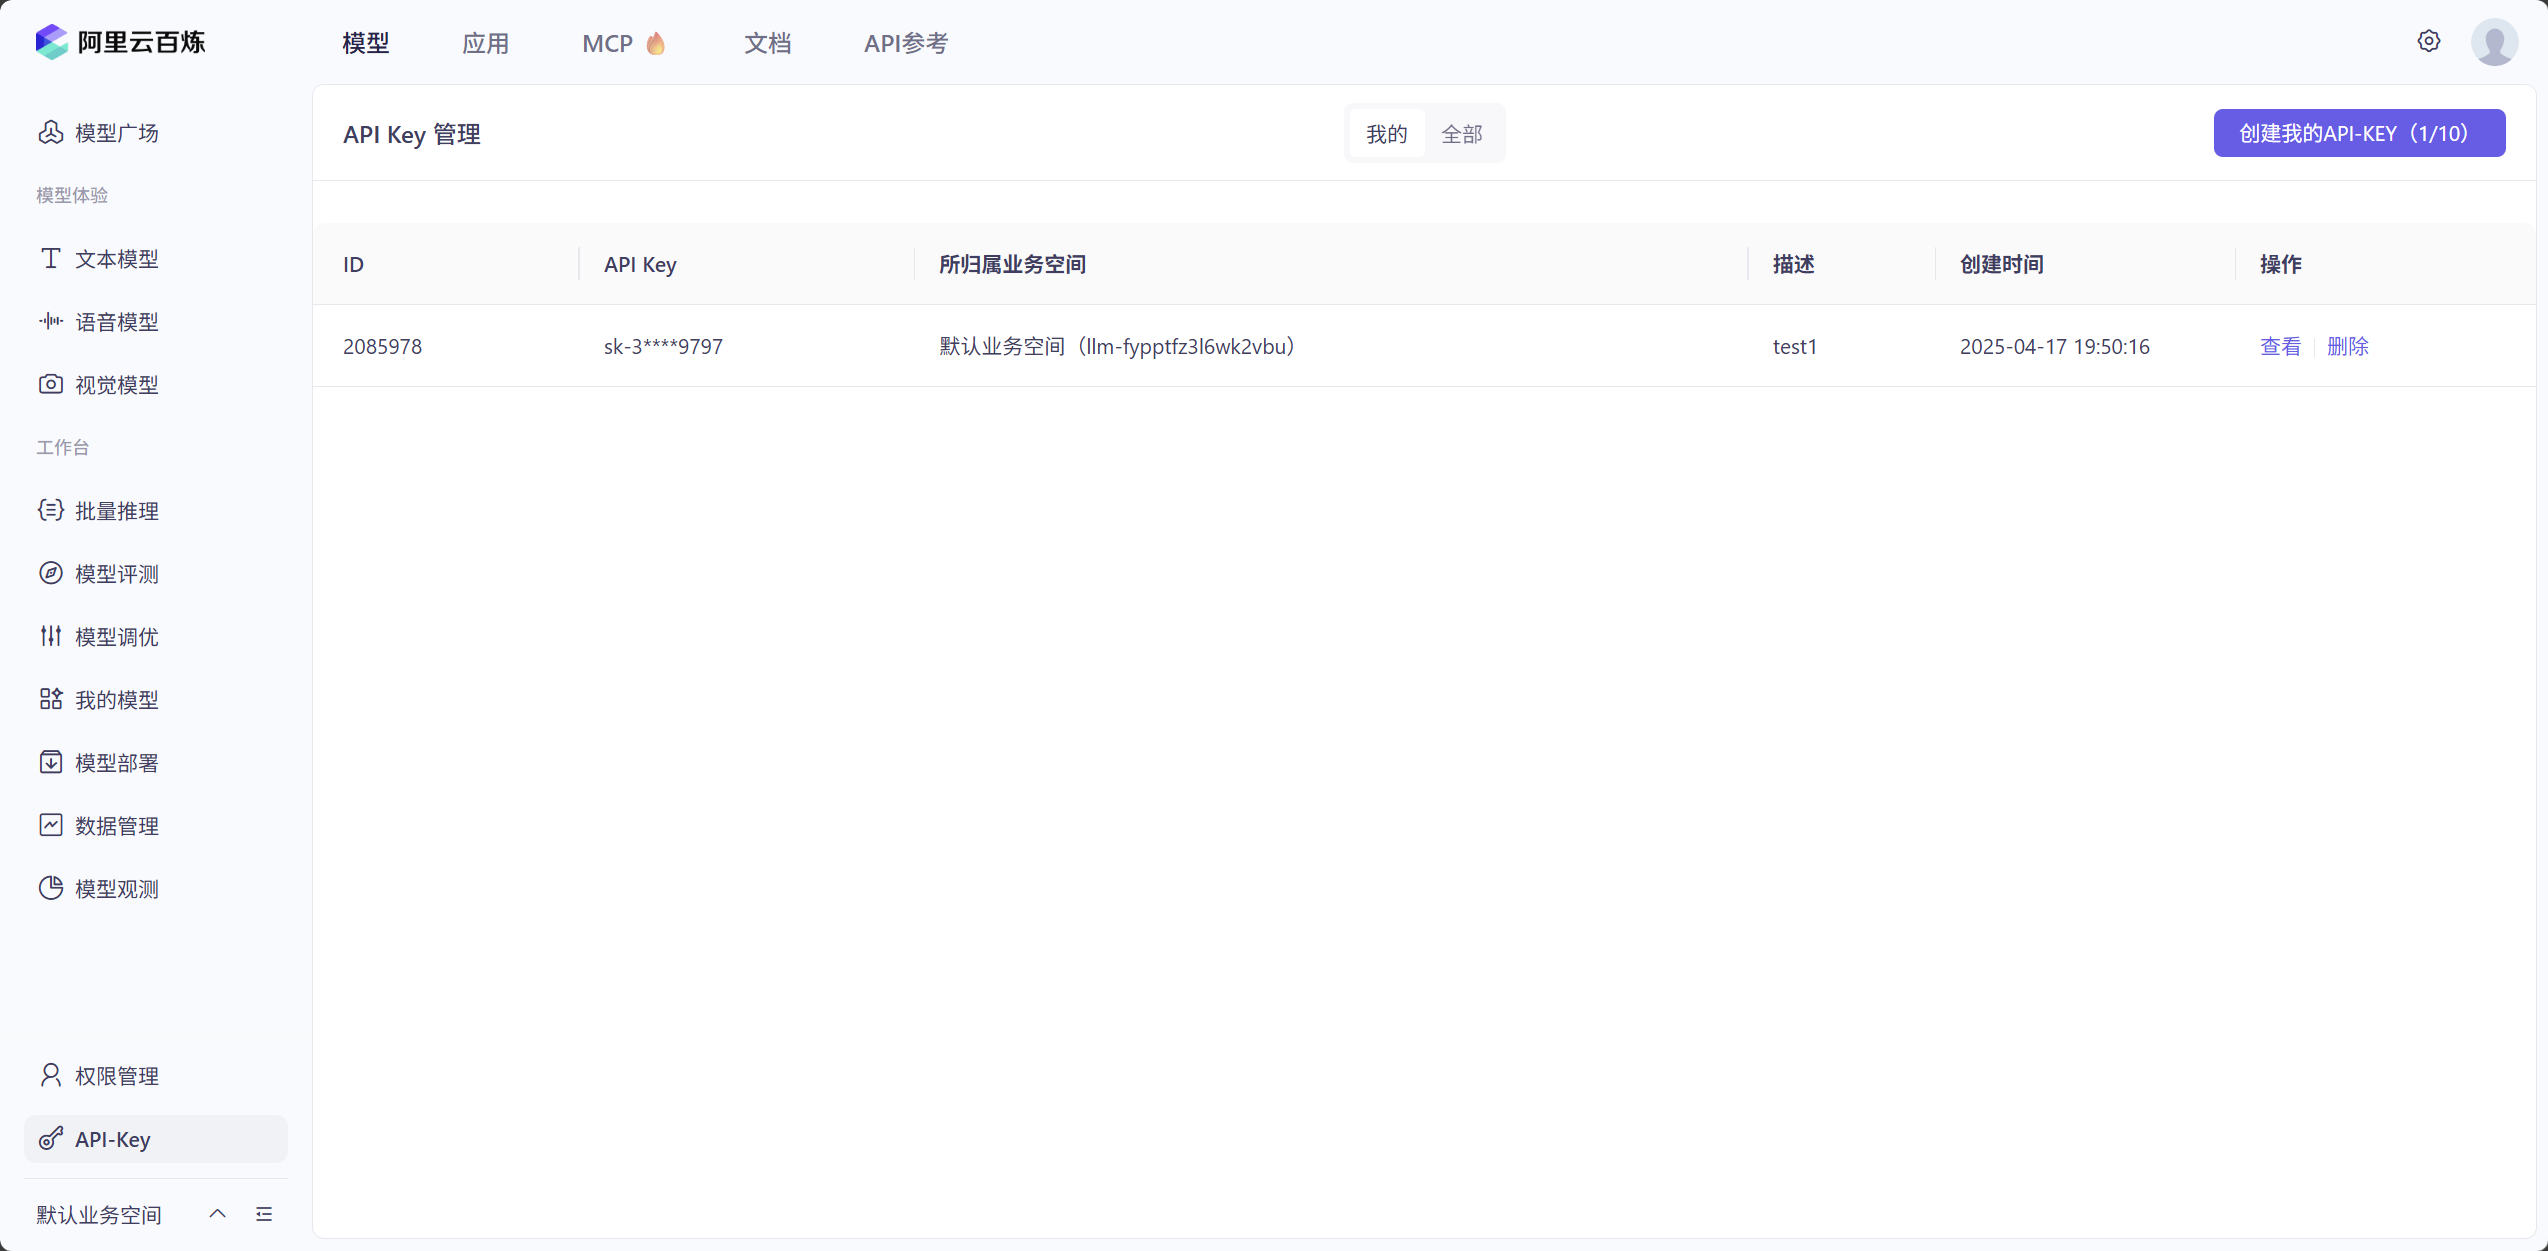
\includegraphics[width=11cm]{./images/13.创建api.png}
		\caption{创建api}
	\end{figure}
	
	由于涉及隐私问题,此处不展示api的具体内容
	
	接下来讲api配置到本机的环境变量内
	
	\begin{figure}[H]
		\centering
		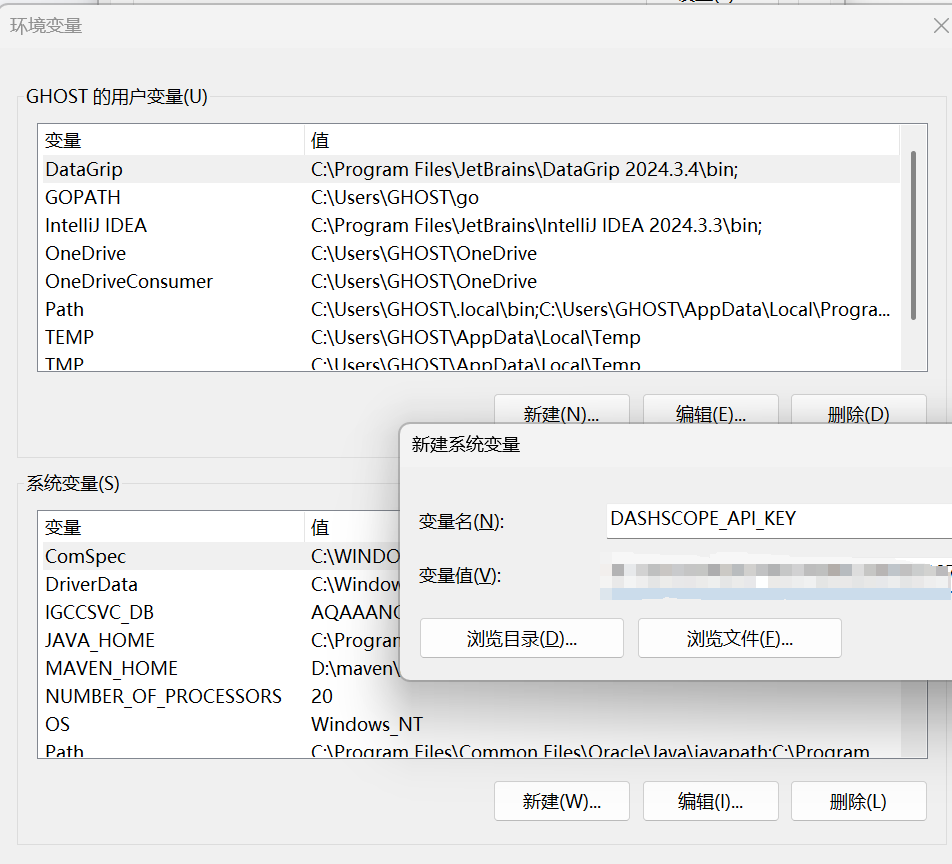
\includegraphics[width=11cm]{./images/14.配置环境变量.png}
		\caption{配置环境变量}
	\end{figure}
	
	在命令行中输入以下命令,检查是否添加完毕
	
	\begin{lstlisting}[language=bash, title=uv安装, tabsize=4]
		echo %DASHSCOPE_API_KEY%
	\end{lstlisting}
	
	\begin{figure}[H]
		\centering
		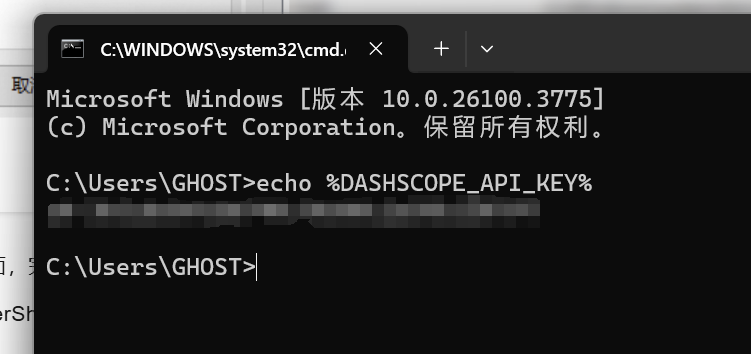
\includegraphics[width=11cm]{./images/15.检查环境变量.png}
		\caption{检查环境变量}
	\end{figure}
	
	\subsection{修改配置文件}
	
	根据参考文档,我们用的是tongyi就配置configs下的proxy-tongyi.toml
	
	\begin{enumerate}[noitemsep, label={\arabic*.}]
		\item 将配置好的api写入配置文件的api\_keys部分
		\begin{enumerate}[noitemsep, label={\arabic{enumi}.\arabic*}]
			\item 可以写成:api\_key = "\${env:DASHSCOPE\_API\_KEY:TONGYI\_API\_KEY}"的格式
			\item 也可以写成:api\_key = {your\_api\_key}
			\item 由于涉及隐私保护,推荐使用调用环境变量的方法
		\end{enumerate}\textbf{}
		\item 配置Server的端口等信息
		\item rag我们暂时不需要可以先不配置
	\end{enumerate}\textbf{}
	
	完整的配置信息如下:
	
	\begin{lstlisting}[title=dbgpt-proxy-tongyi.toml, tabsize=4]
	[system]
	# Load language from environment variable(It is set by the hook)
	language = "${env:DBGPT_LANG:-zh}"
	api_keys = []
	encrypt_key = "your_secret_key"
	
	# Server Configurations
	[service.web]
	host = "0.0.0.0"
	port = 5670
	
	[service.web.database]
	type = "sqlite"
	path = "pilot/meta_data/dbgpt.db"
	
	[rag.storage]
	[rag.storage.vector]
	type = "chroma"
	persist_path = "pilot/data"
	
	# Model Configurations
	[models]
	[[models.llms]]
	name = "qwen-plus"
	# provider = "${env:LLM_MODEL_PROVIDER:proxy/tongyi}"
	provider = "proxy/openai"
	api_base = "https://dashscope.aliyuncs.com/compatible-mode/v1"
	api_key = "${env:DASHSCOPE_API_KEY}"
	
	[[models.embeddings]]
	name = "text-embedding-v3"
	# provider = "${env:EMBEDDING_MODEL_PROVIDER:proxy/tongyi}"
	provider = "proxy/openai"
	api_url = "https://dashscope.aliyuncs.com/compatible-mode/v1/embeddings"
	api_key = "${env:DASHSCOPE_API_KEY}"
	\end{lstlisting}
	
	\subsection{启动项目}
	
	\begin{lstlisting}[language=bash, title=uv安装, tabsize=4]
		uv run --no-project python packages/dbgpt-app/src/dbgpt_app/dbgpt_server.py --config configs/dbgpt-proxy-tongyi.toml
	\end{lstlisting}
	
	这里我们经常会遇到以下报错:
	
	\begin{tcolorbox}[colback = red!25!white, colframe = red!75!black]
		error: Failed to fetch: `https://pypi.org/simple/charset-normalizer/`
		
		Caused by: request or response body error
		
		Caused by: operation timed out
	\end{tcolorbox}
	
	
	这是由于没有连接上,多尝试几次即可
	
	重新运行,得到以下结果:表示成功
	
	\begin{figure}[H]
		\centering
		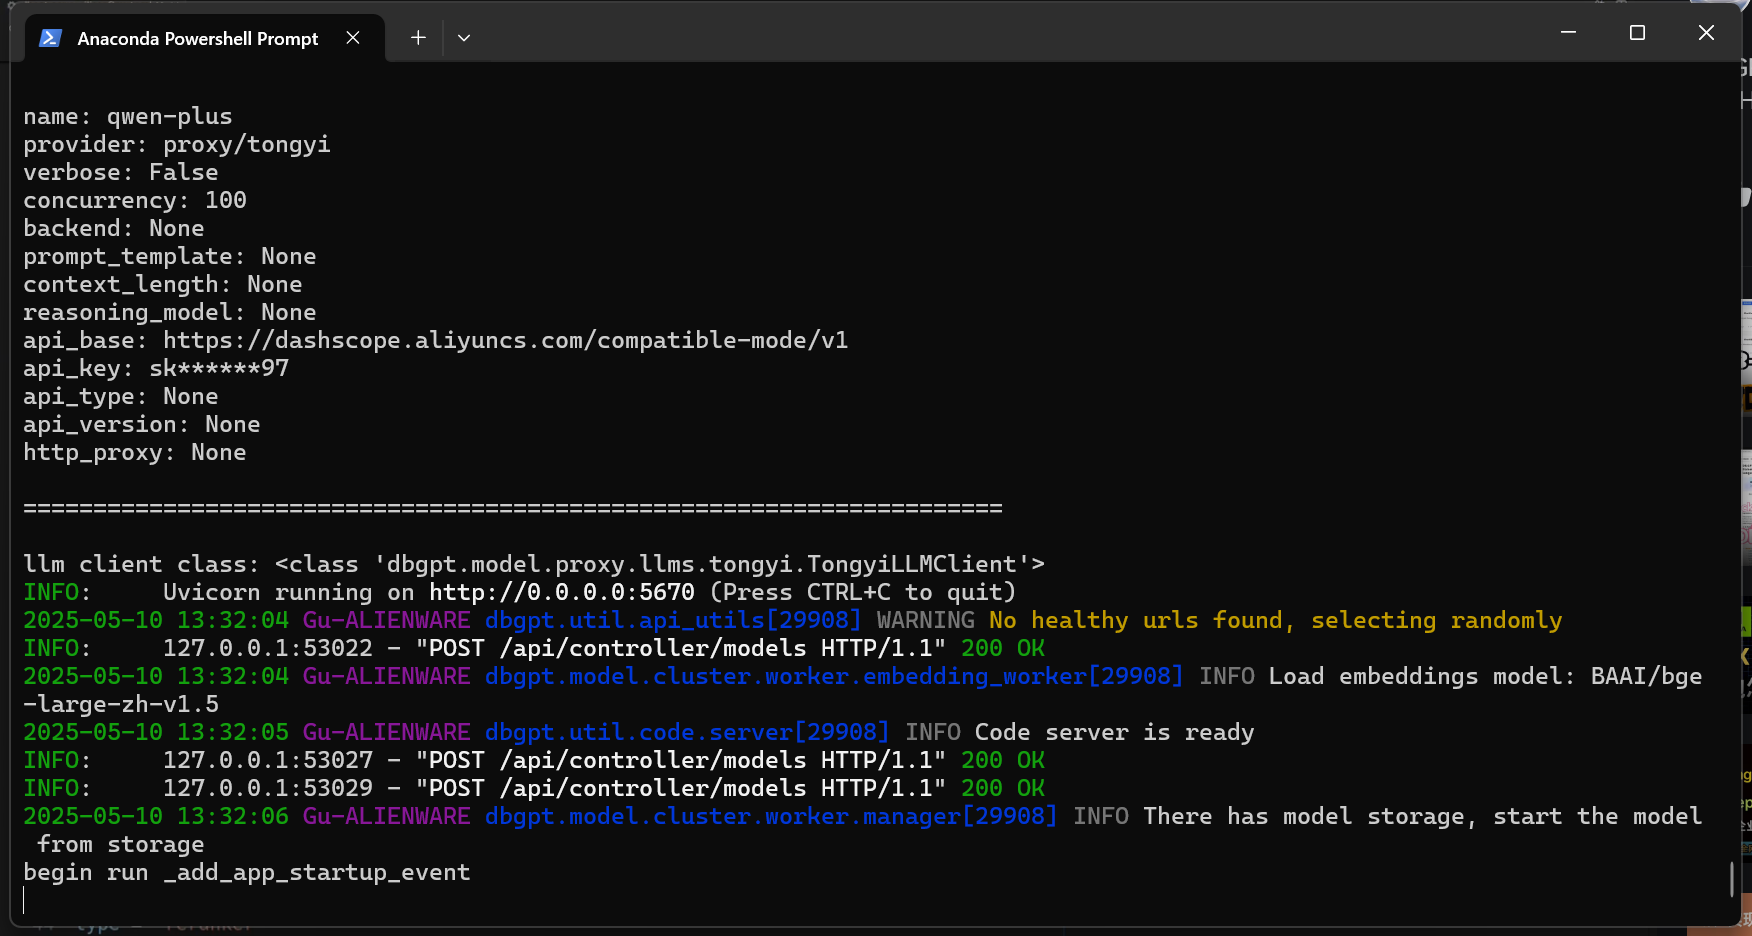
\includegraphics[width=11cm]{./images/16.运行成功.png}
		\caption{运行成功}
	\end{figure}
	
	浏览器输入:127.0.0.1:5670,可以看到DB-GPT页面:
	
	\begin{figure}[H]
		\centering
		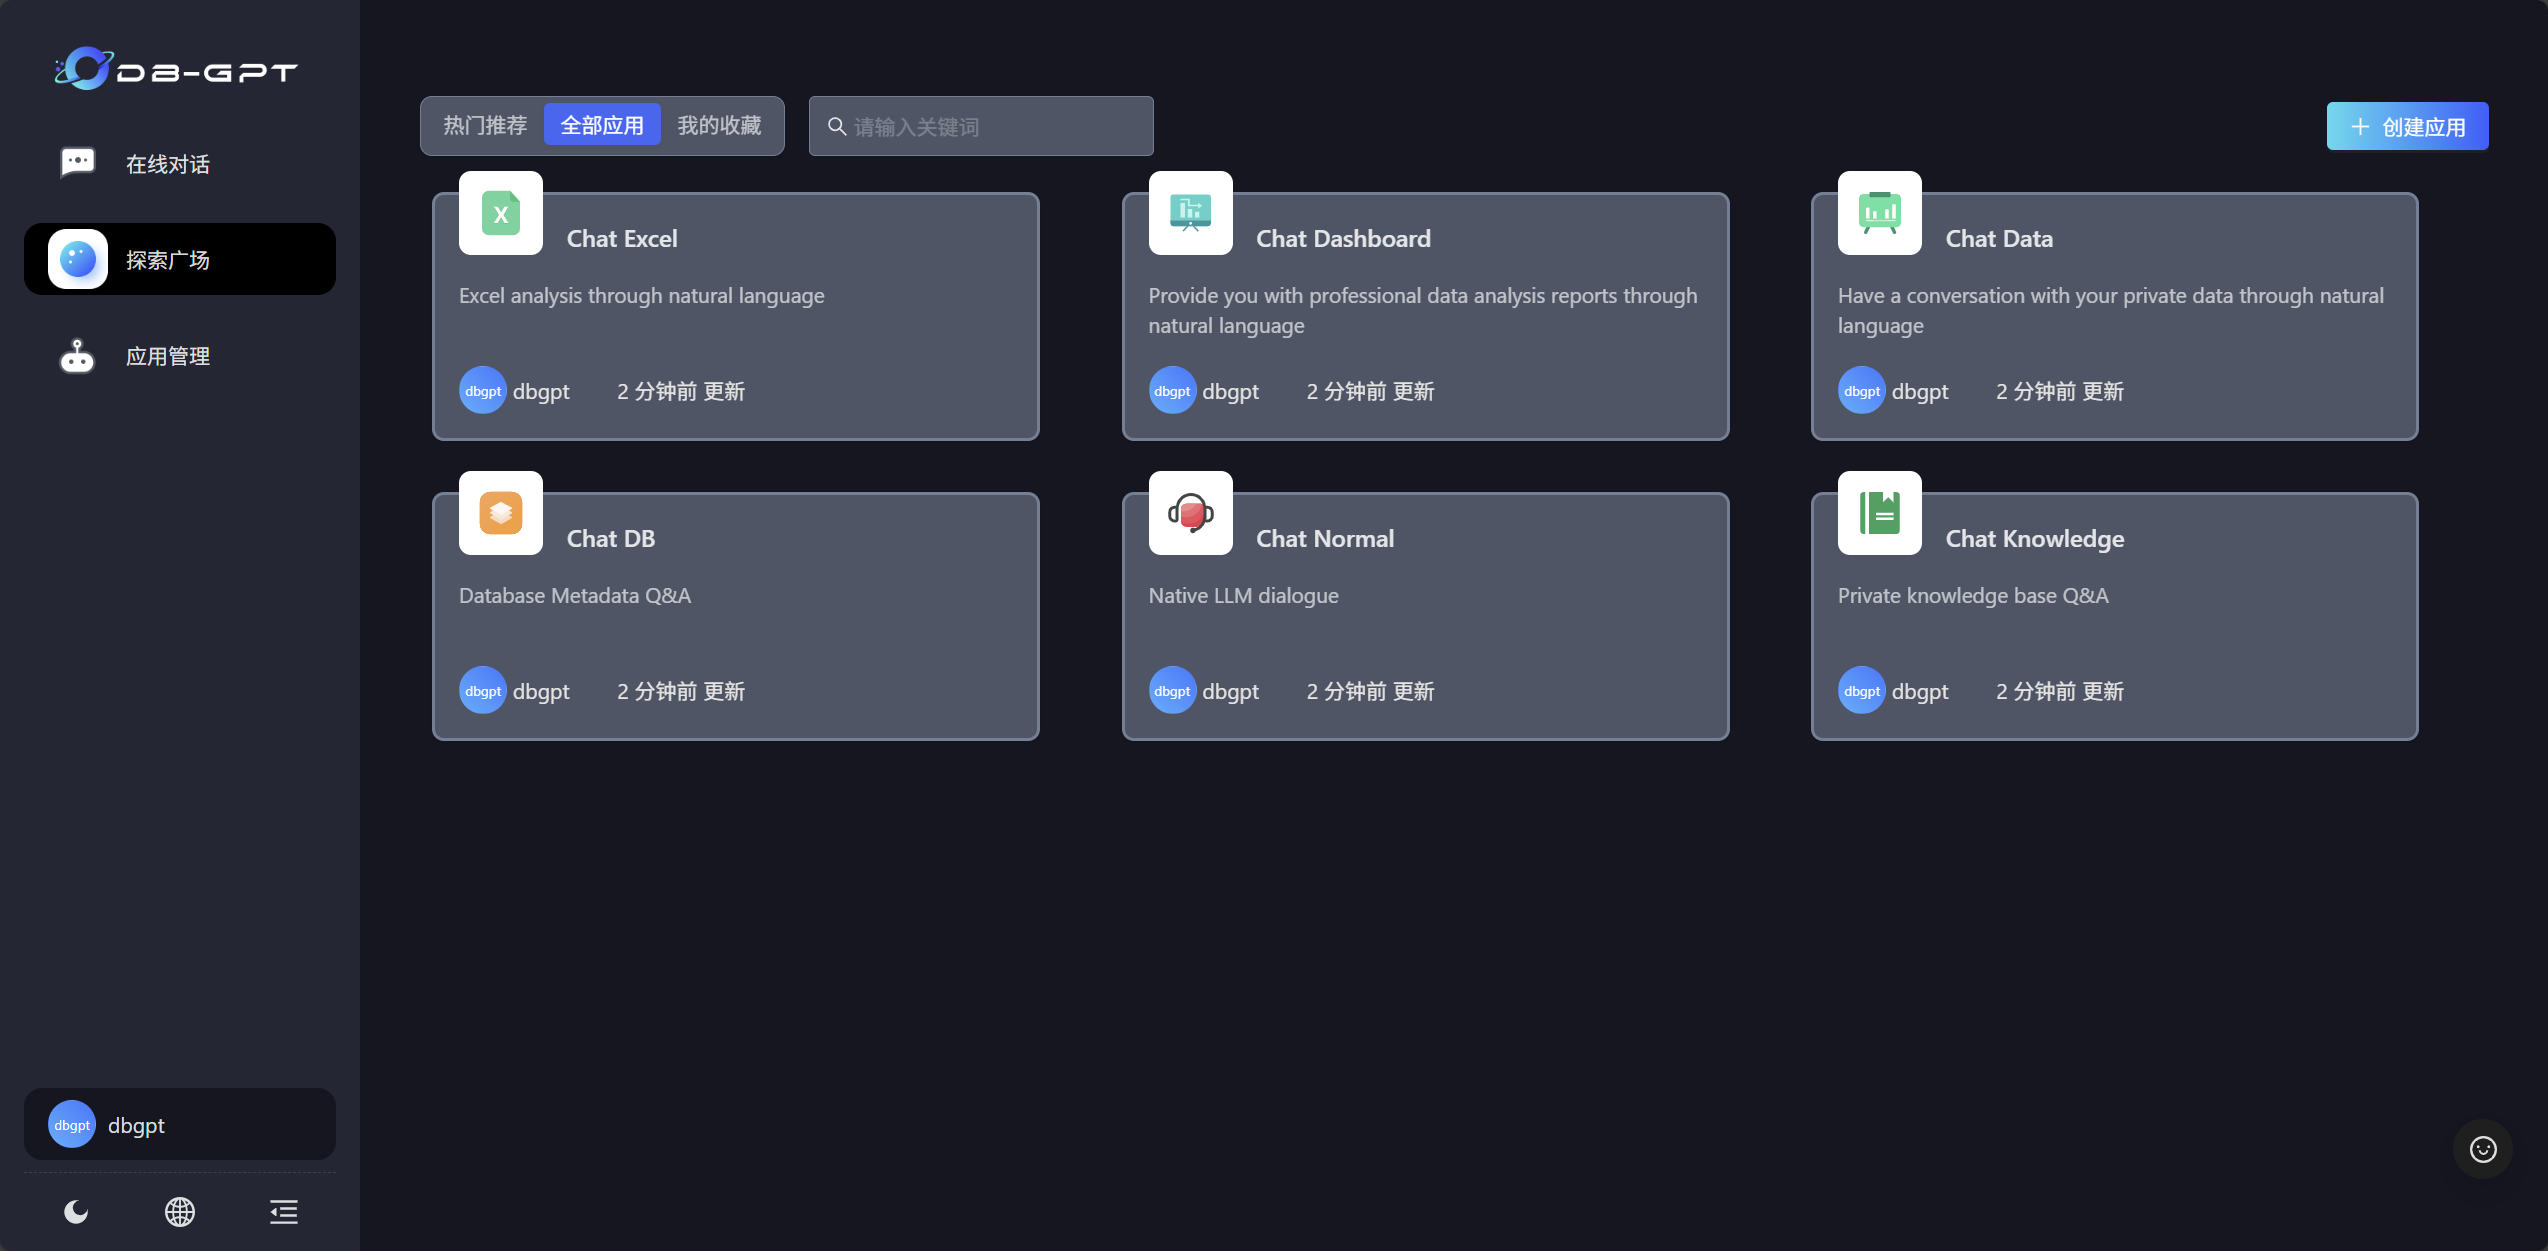
\includegraphics[width=11cm]{./images/17.DB-GPT页面.png}
		\caption{DB-GPT页面}
	\end{figure}
	
	在“应用管理” –> “模型管理”里可以看到:刚刚配置好的qwen-plus
	
	\begin{figure}[H]
		\centering
		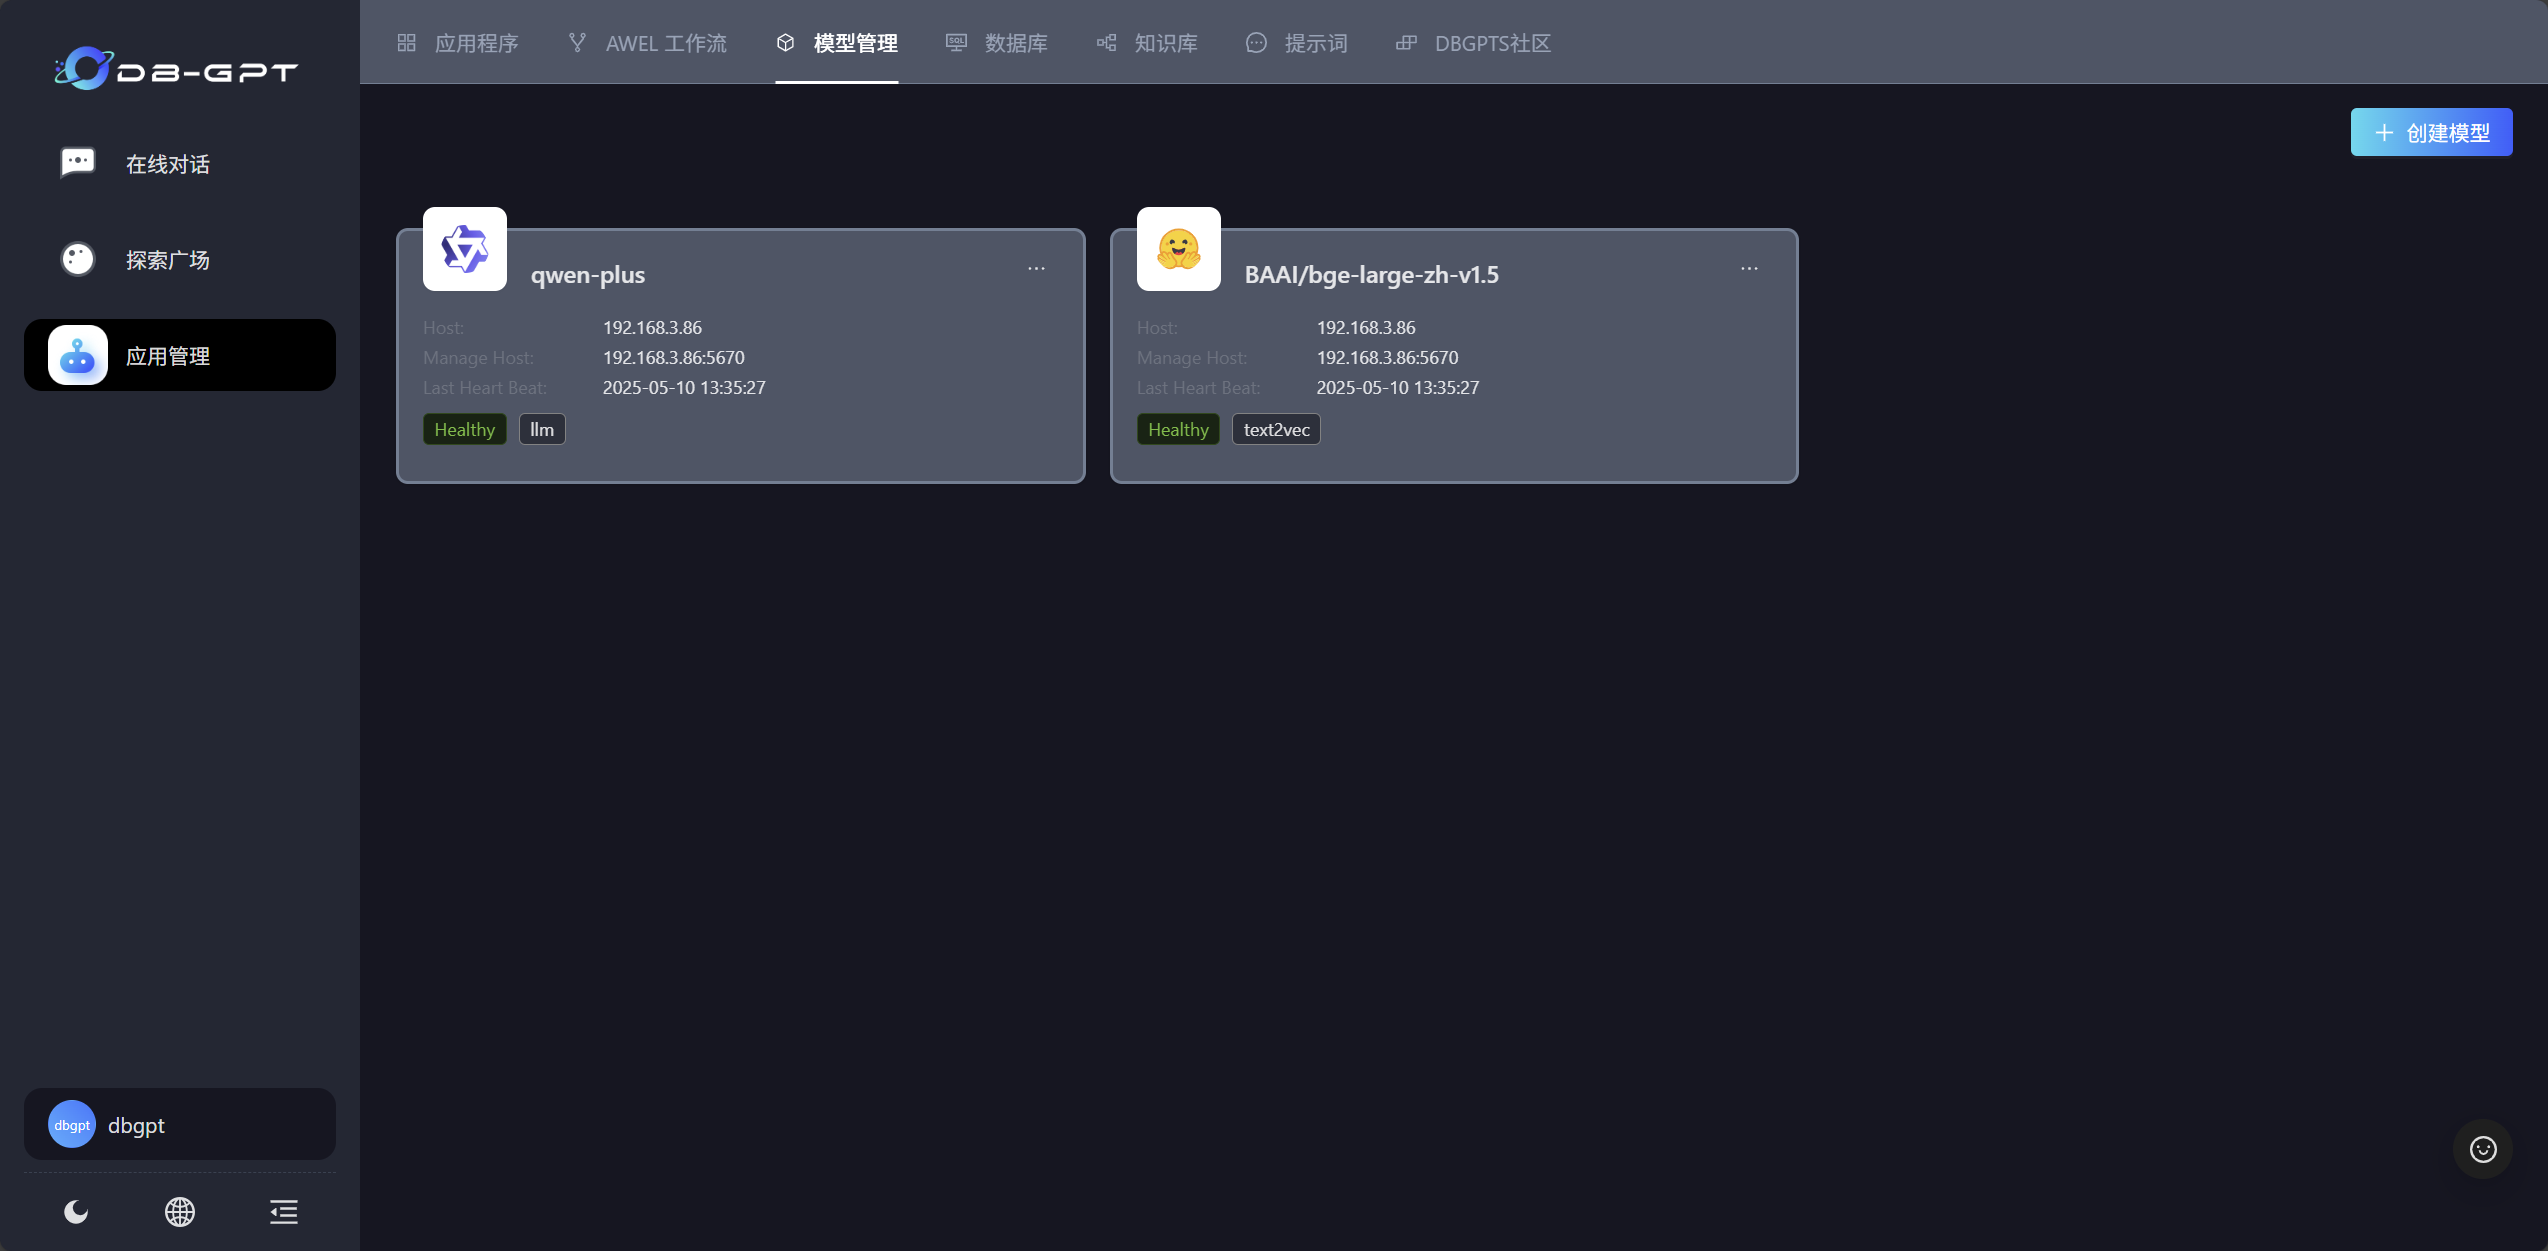
\includegraphics[width=11cm]{./images/18.qwen-plus.png}
		\caption{qwen-plus}
	\end{figure}
	
	我们这里先用在线对话来测试一下,给qwen-plus发送一句你好
	
	可以从conda与网页里看到:发送以及回复的消息:
	
	\begin{figure}[H]
		\centering
		\begin{minipage}[b]{0.45\textwidth}
			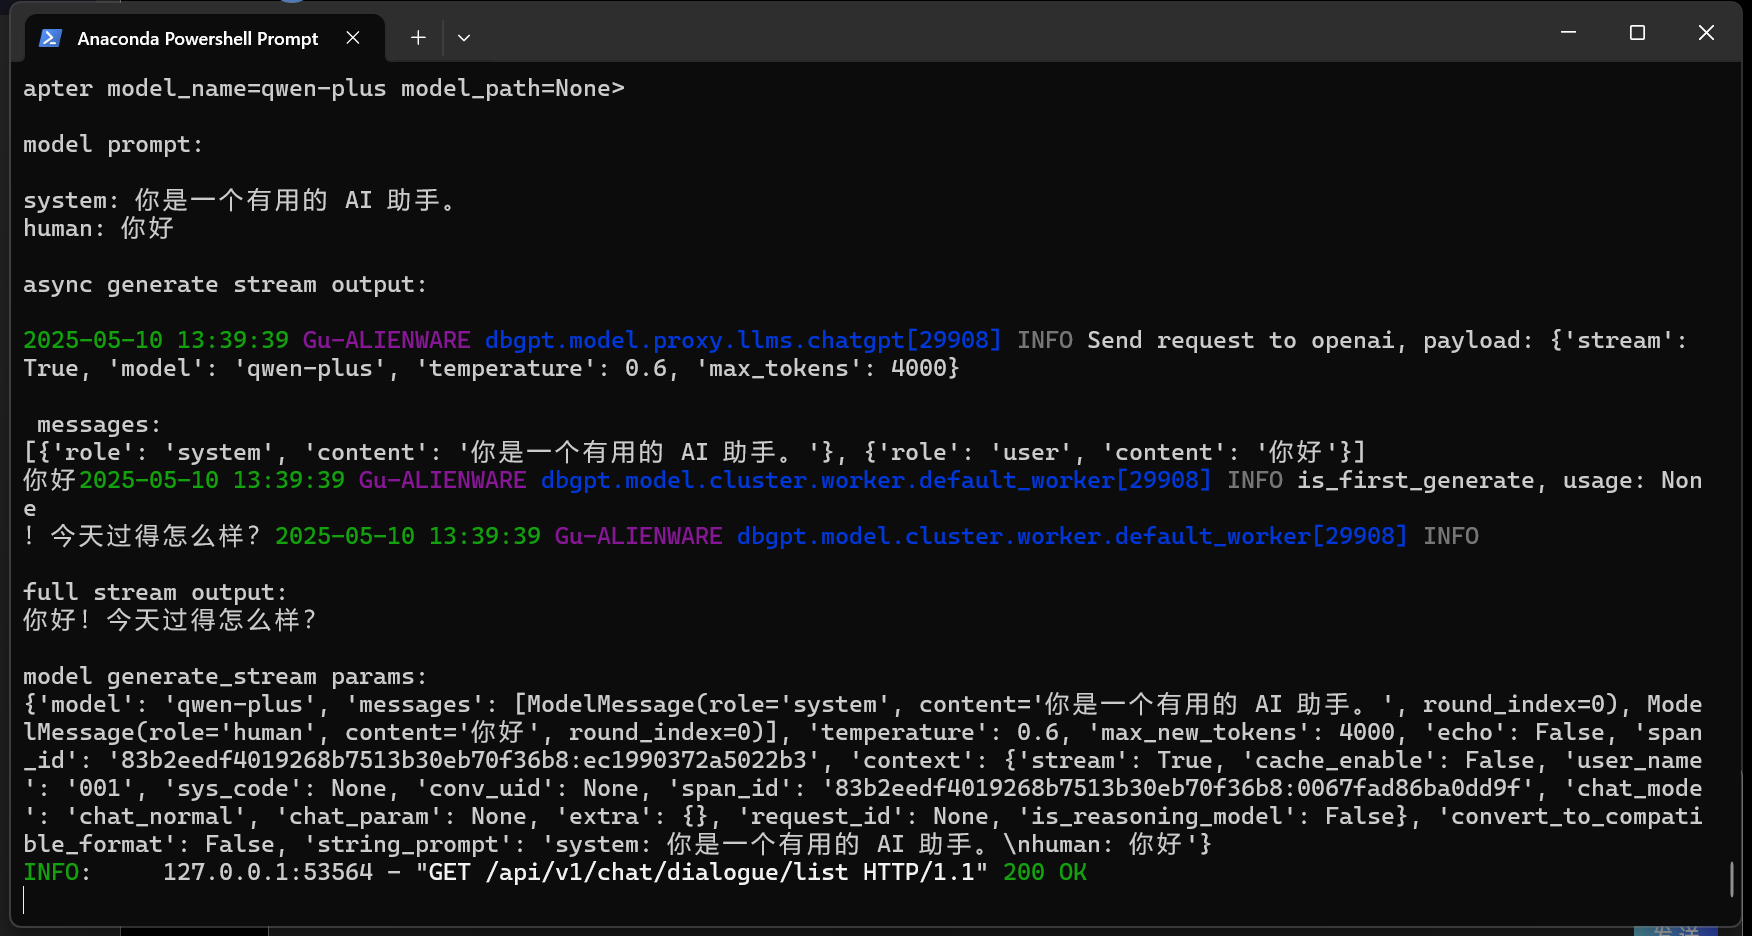
\includegraphics[width=\textwidth]{./images/19.发送“你好”-后台.png}
			\caption{发送“你好”-后台}
		\end{minipage}
		\hfill
		\begin{minipage}[b]{0.45\textwidth}
			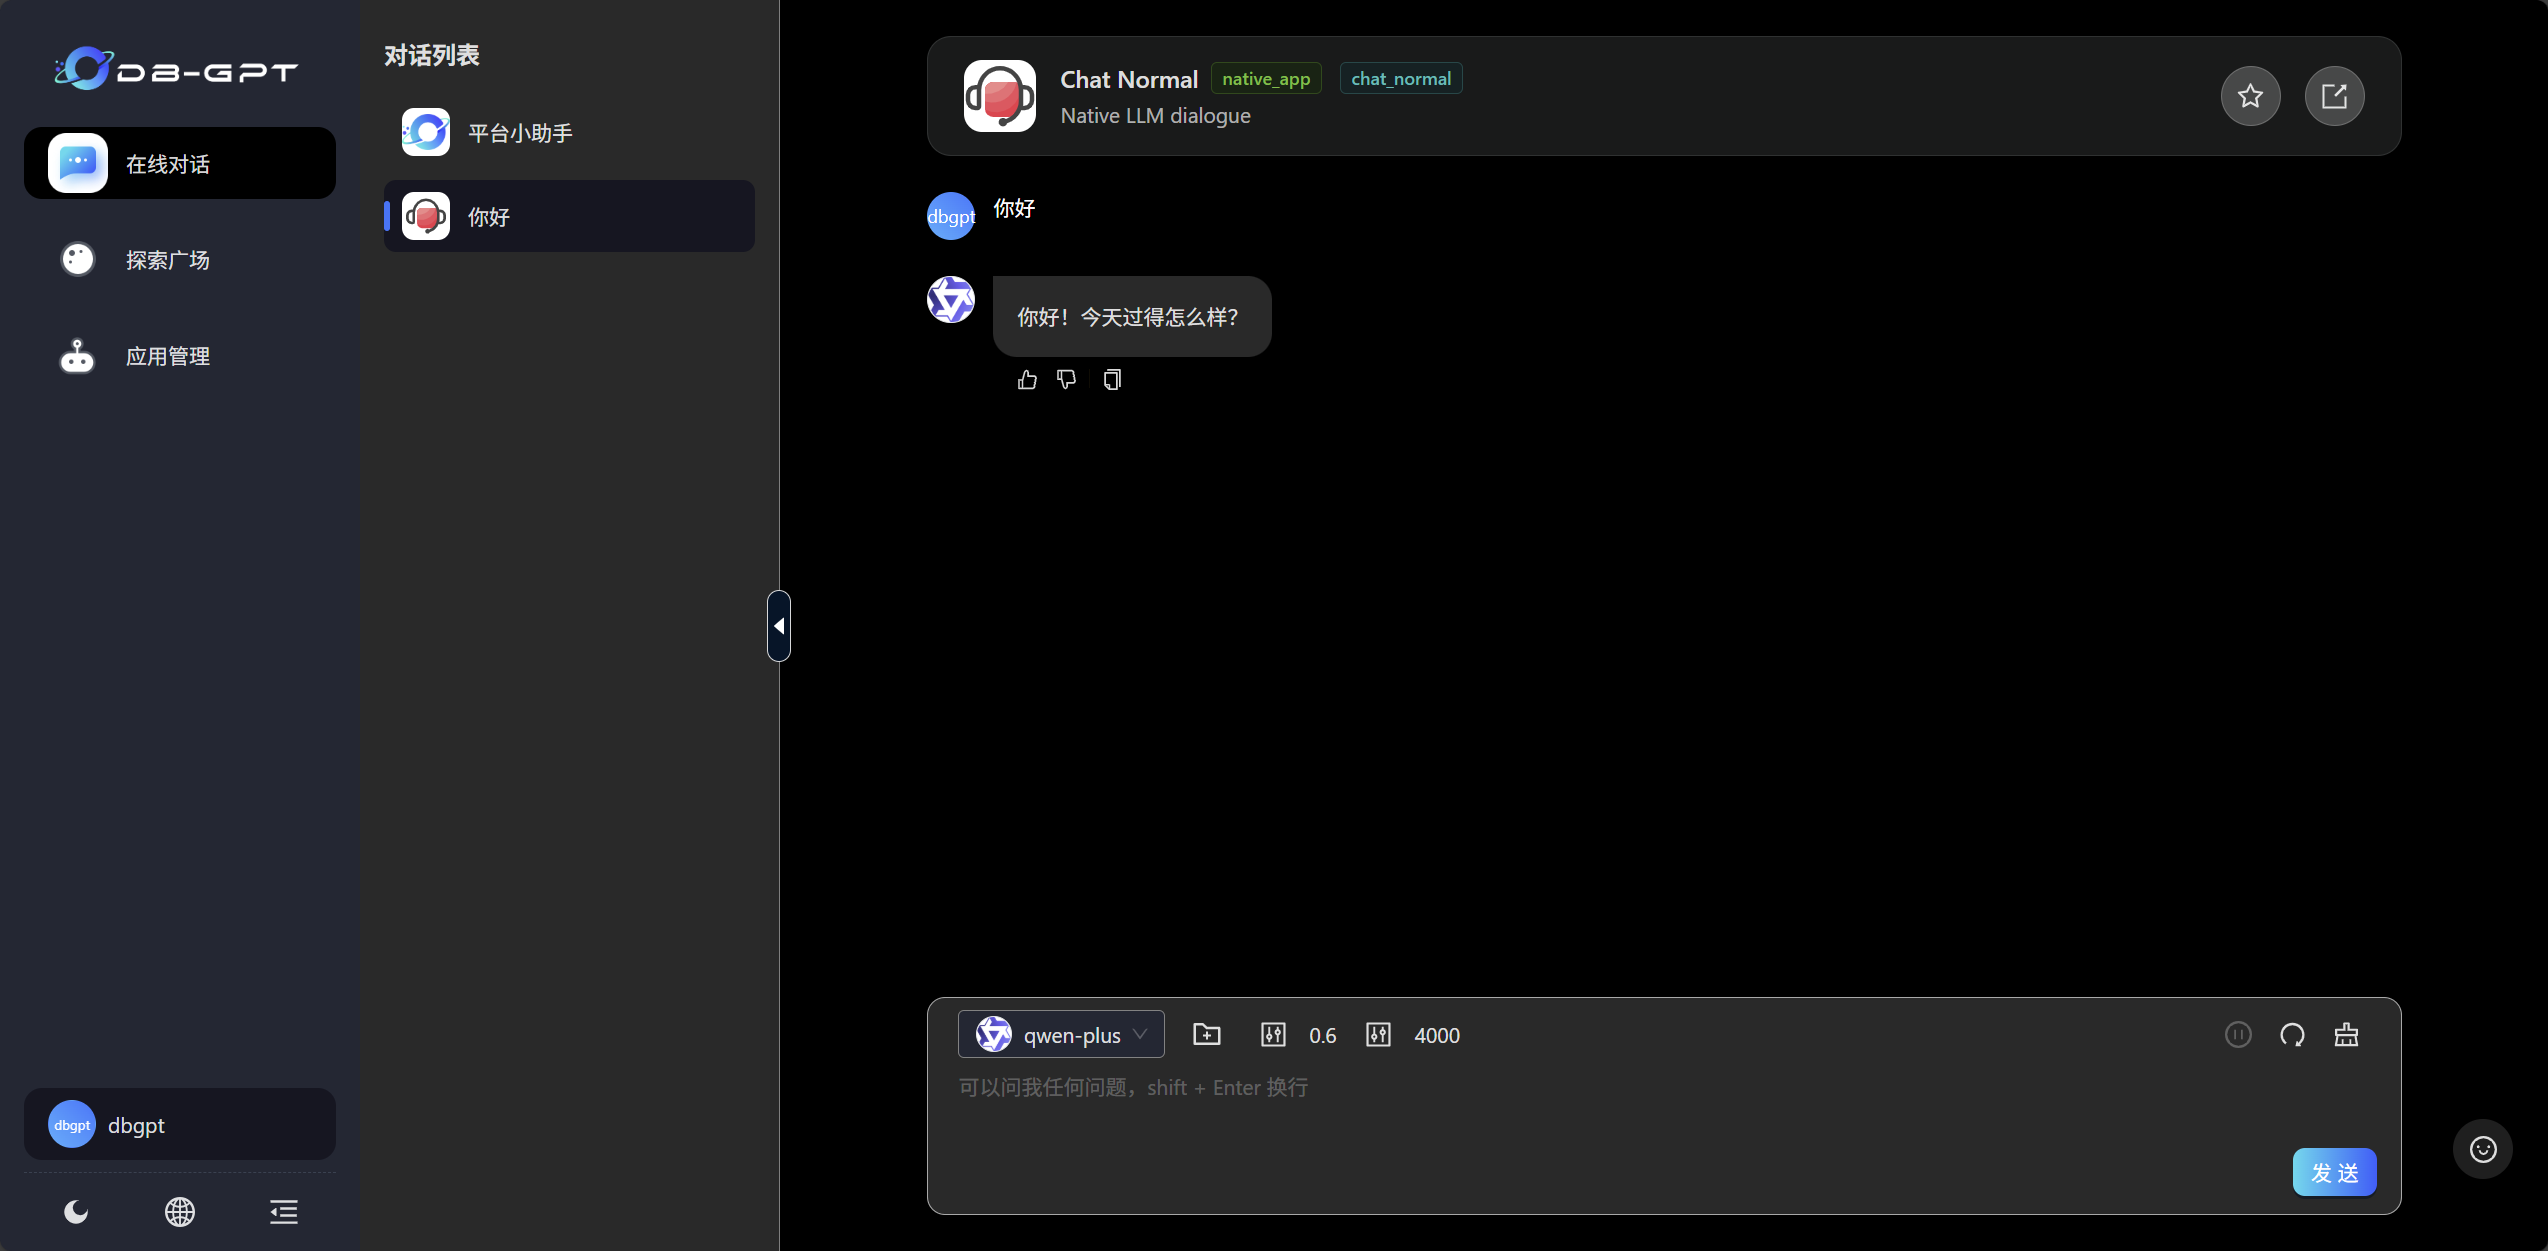
\includegraphics[width=\textwidth]{./images/20.发送“你好”-网页.png}
			\caption{发送“你好”-网页}
		\end{minipage}
	\end{figure}
	
	\subsection{添加数据库}
	
	在 应用广场 –> 数据库 -> 添加数据库,选择sqlite并导入提供的数据库
	
	\begin{figure}[H]
		\centering
		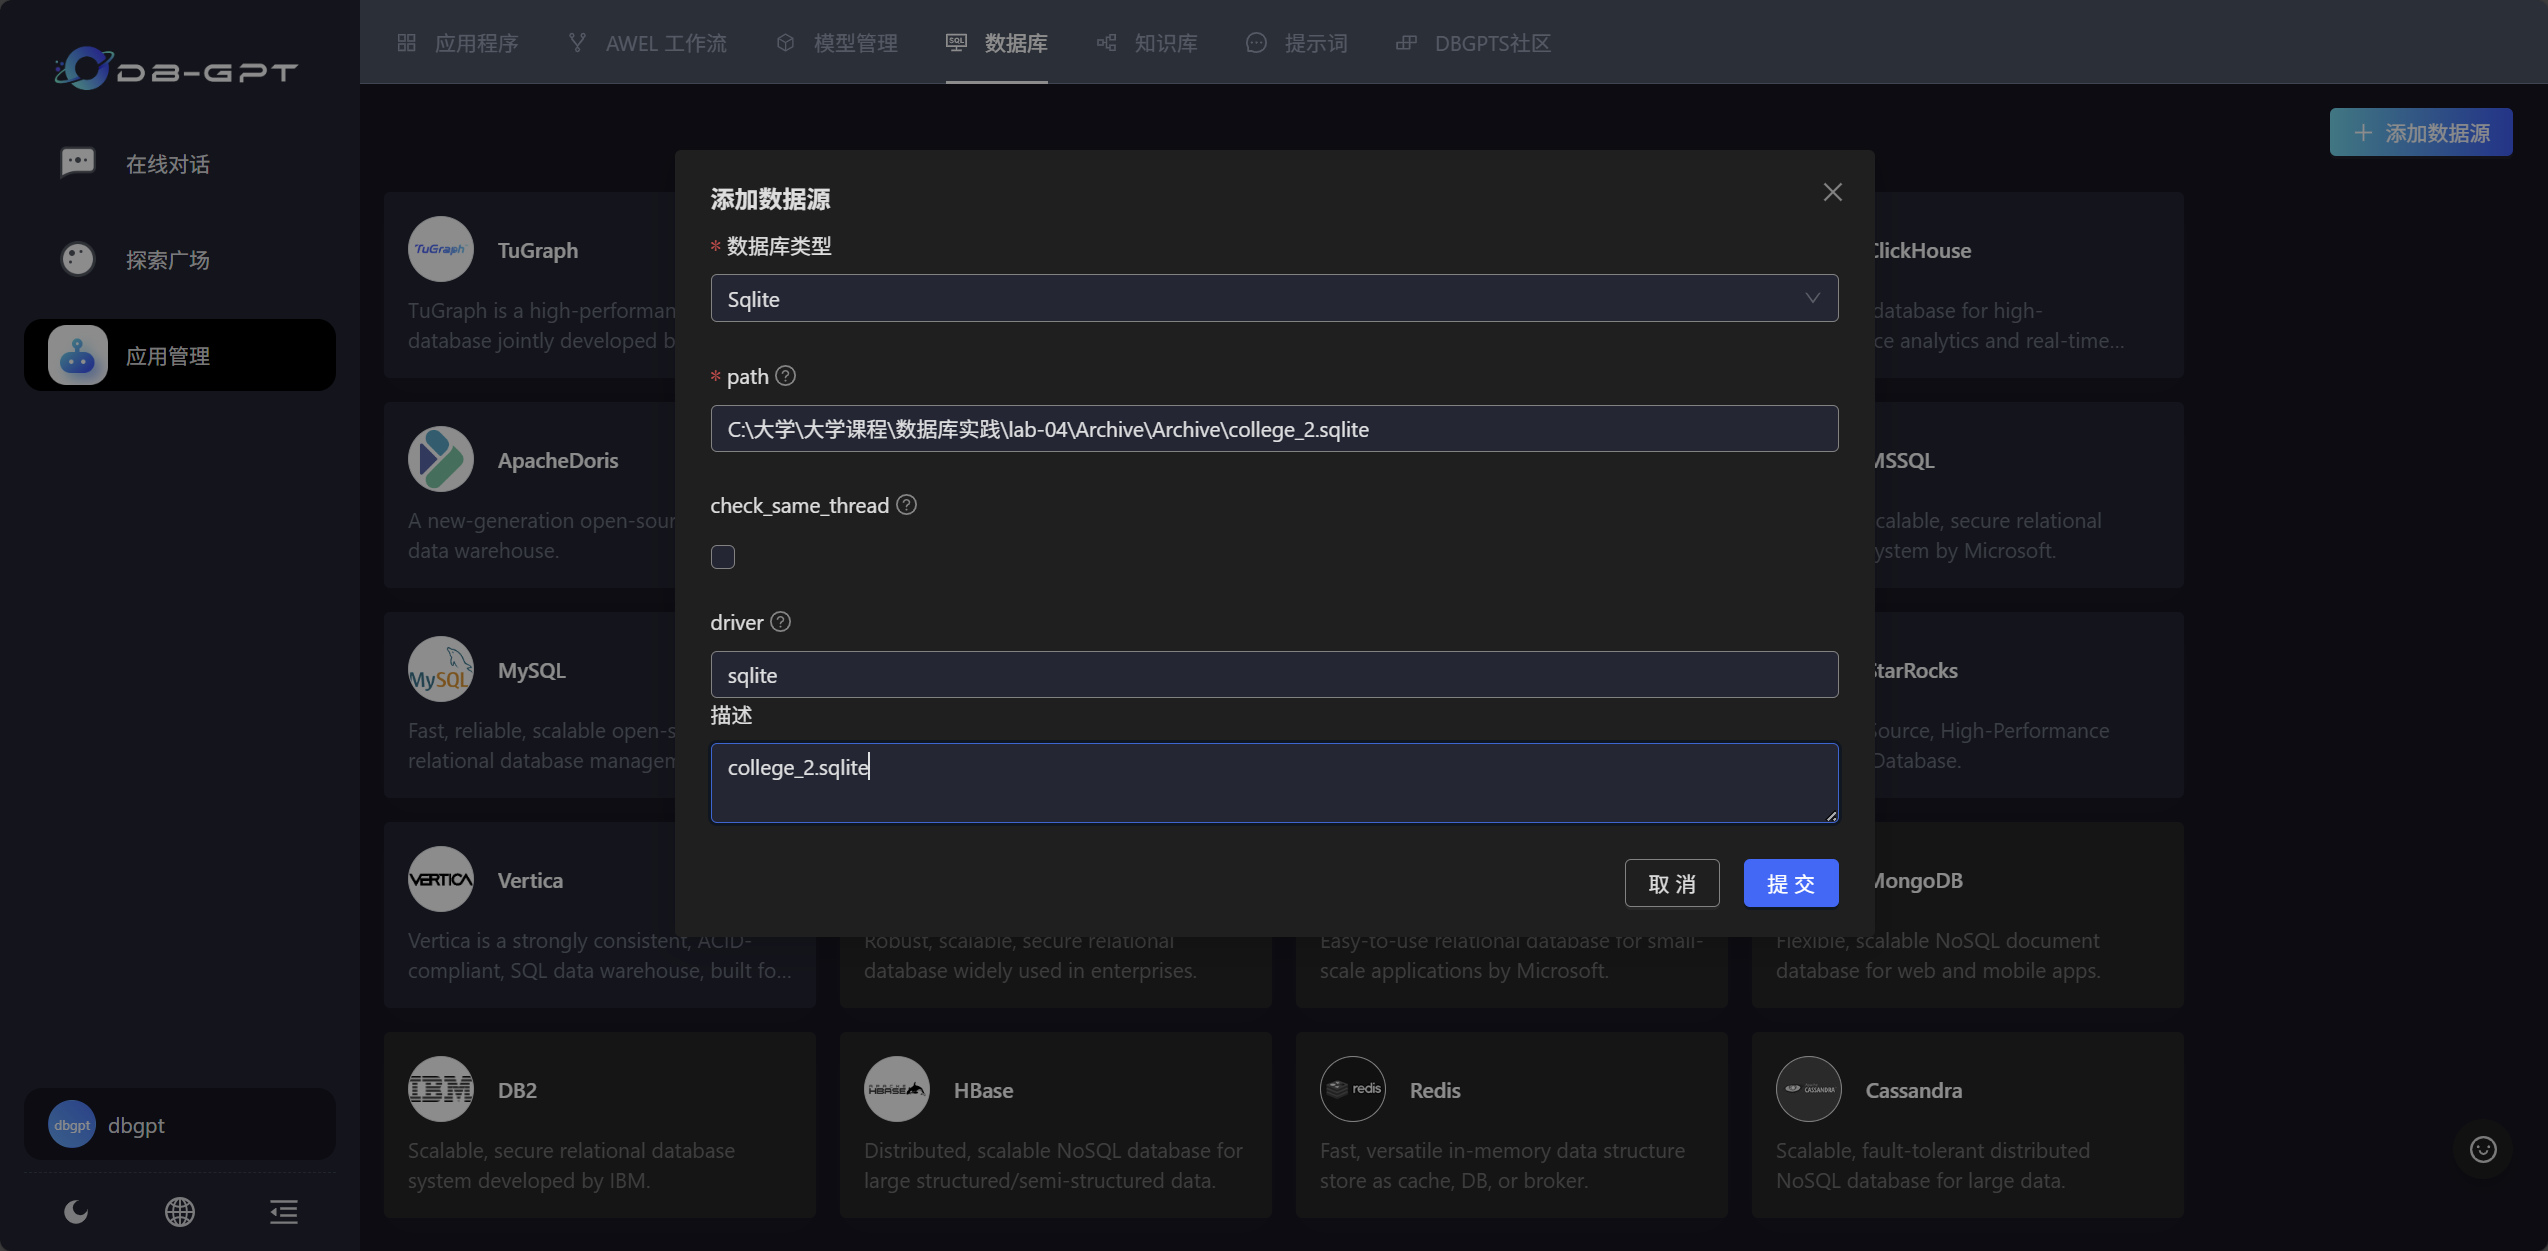
\includegraphics[width=9cm]{./images/21.添加数据库.png}
		\caption{添加数据库}
	\end{figure}
	
	在chat-data中加入数据库,看到以下内容表示导入成功:
	
	\begin{figure}[H]
		\centering
		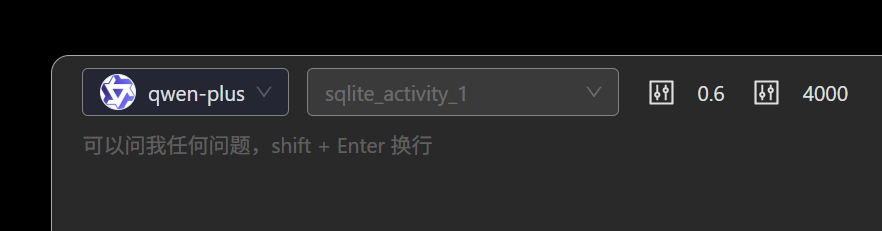
\includegraphics[width=11cm]{./images/22.添加数据库成功.png}
		\caption{添加数据库成功}
	\end{figure}
	
	\section{开始提问}
	
	我选择了基于两个数据库的:Lab-1的作业内容、图形化展示问题、数据分析问题,全部问题如下:
	
	\begin{enumerate}[noitemsep, label={\arabic*.}]
		\item 基于 sqlite\_activity\_1 的 SQL 编写的问题
		\begin{enumerate}[noitemsep, label={\alph*.}]
			\item 如何编写 SQL 语句来获取参与任何活动的教师人数?
			\item 如何用 SQL 查询 Mark Giuliano 参与了多少项活动?
			\item 如何编写 SQL 语句来获取指导学生最多的教师的姓和名?
		\end{enumerate}
		
		\item 基于 sqlite\_activity\_1 的图形化展示的问题
		\begin{enumerate}[noitemsep, label={\alph*.}]
			\item 绘制一张柱状图,展示每个建筑中的教师人数。
			\item 绘制一张饼图,展示不同活动名称的学生参与人数。
		\end{enumerate}
		
		\item 基于 sqlite\_college\_2 的 SQL 编写的问题
		\begin{enumerate}[noitemsep, label={\alph*.}]
			\item 如何编写 SQL 语句来列出所有课程的名称,并按课程标题和学分排序?
			\item 如何用 SQL 查询物理系提供的不同课程数量?
		\end{enumerate}
		
		\item 基于 sqlite\_college\_2 的图形化展示的问题
		\begin{enumerate}[noitemsep, label={\alph*.}]
			\item 用统计图展示各部门的教师数量及其平均薪水。
			\item 用统计图展示各个教师授课课程的数量。
			\item 如何用饼图展示不同年级、不同学期的课程选修人数占总选修人数的比例?
		\end{enumerate}
		
		\item 基于 sqlite\_college\_2 的数据分析类的问题
		\begin{enumerate}[noitemsep, label={\alph*.}]
			\item 如何分析教师的授课负担?(例如,哪些教师在多个学期中教授了大量课程?)
			\item 如何找出哪些课程是核心课程?(例如,这些课程连续开设了多年?)
		\end{enumerate}
	\end{enumerate}
	
	\subsection{问题1}
	
	如何编写SQL语句来获取参与任何活动的教师人数?
	
	\begin{figure}[H]
		\centering
		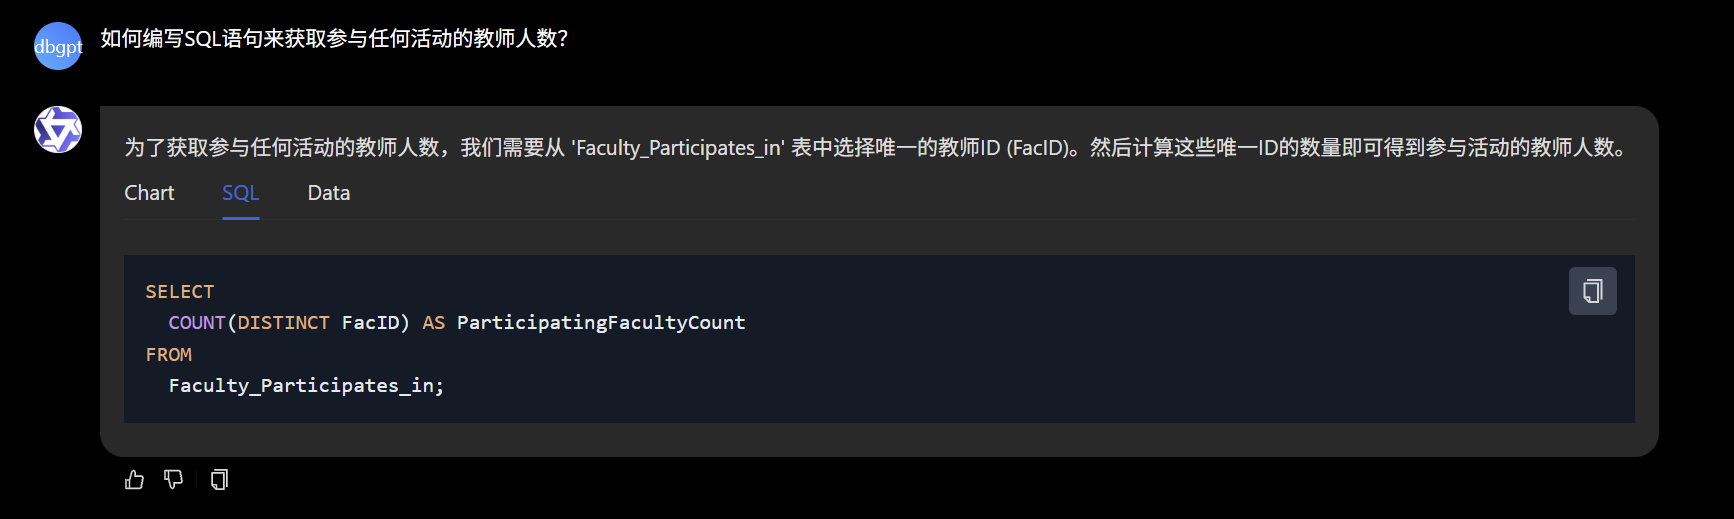
\includegraphics[width=11cm]{./images/23.问题1.png}
		\caption{问题1}
	\end{figure}
	
	得到结果:18,与预期一致
	
	\subsection{问题2}
	
	如何用SQL查询Mark Giuliano参与了多少项活动?
	
	\begin{figure}[H]
		\centering
		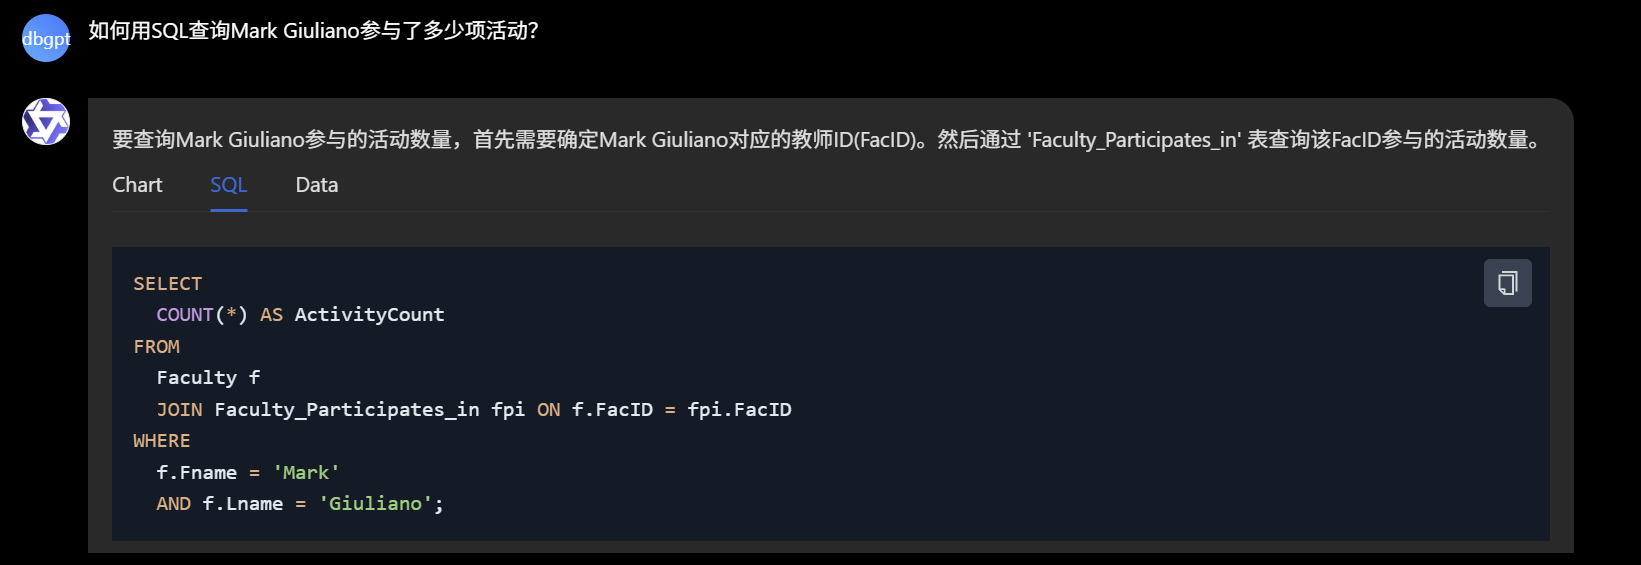
\includegraphics[width=11cm]{./images/24.问题2.png}
		\caption{问题2}
	\end{figure}
	
	得到结果:3,与预期一致
	
	\subsection{问题3}
	如何编写 SQL 语句来获取指导学生最多的教师的姓和名?
	
	\begin{figure}[H]
		\centering
		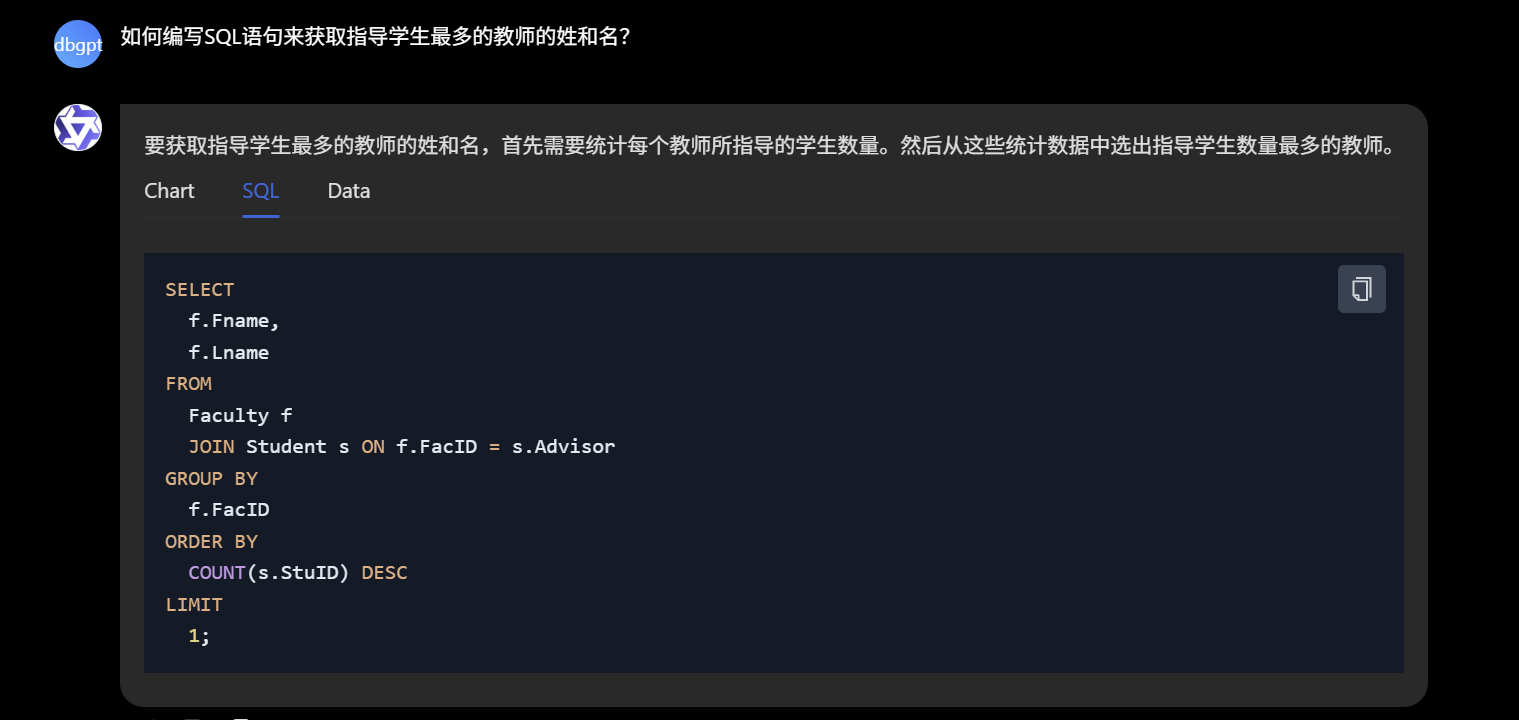
\includegraphics[width=11cm]{./images/25.问题3.png}
		\caption{问题3}
	\end{figure}
	
	得到结果:David, Yarowsky,与预期一致
	
	\subsection{问题4}
	如何绘制一张柱状图,展示每个建筑中的教师人数?
	
	DB-GPT给出了以下语句与结果:
	
	\begin{verbatim}
		SELECT
			Building,
			COUNT(FacID) AS FacultyCount
		FROM
			Faculty
		GROUP BY
			Building;
	\end{verbatim}
	
	\begin{figure}[H]
		\centering
		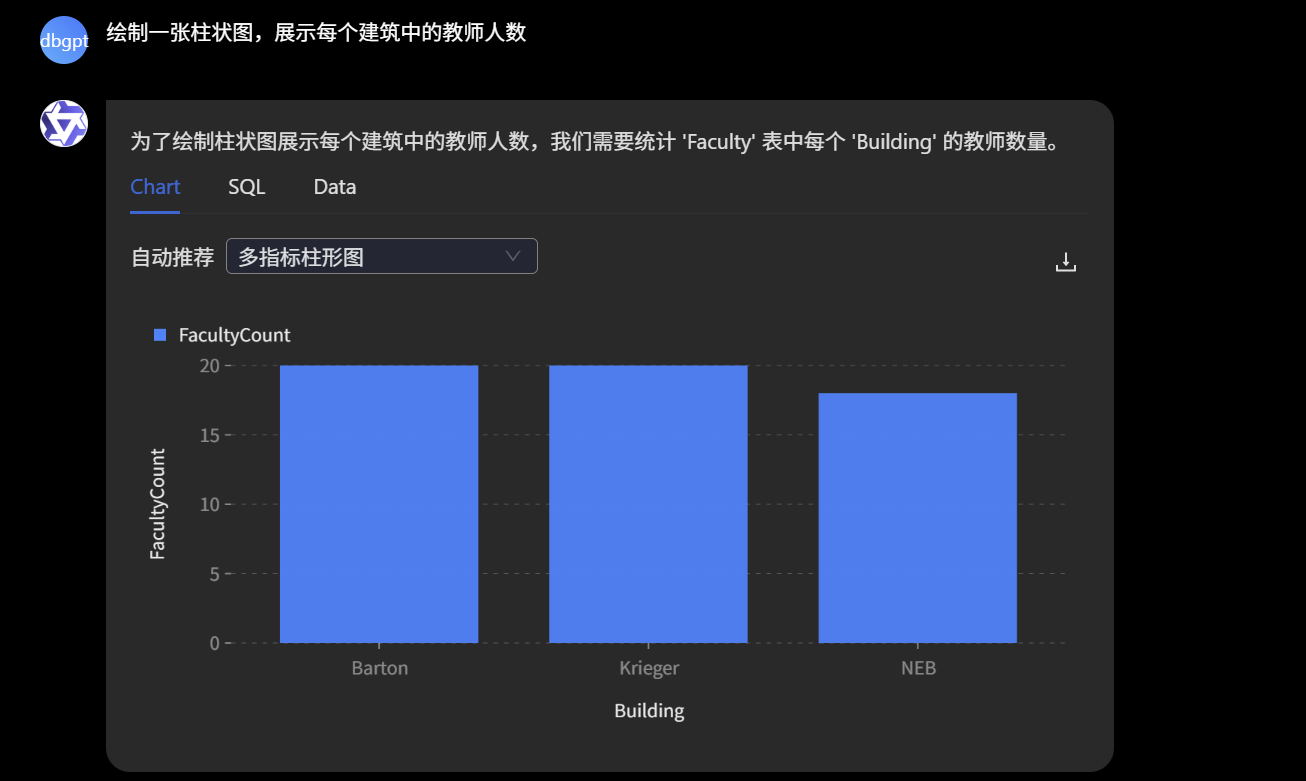
\includegraphics[width=11cm]{./images/26.问题4.png}
		\caption{问题4}
	\end{figure}
	
	\subsection{问题5}
	如何绘制一张饼图,展示不同活动名称的学生参与人数?
	
	DB-GPT给出了以下语句与结果:
	
	\begin{verbatim}
		SELECT
			a.activity_name,
			COUNT(pi.stuid) AS StudentCount
		FROM
			Activity a
			LEFT JOIN Participates_in pi ON a.actid = pi.actid
		GROUP BY
			a.activity_name;
	\end{verbatim}
	
	\begin{figure}[H]
		\centering
		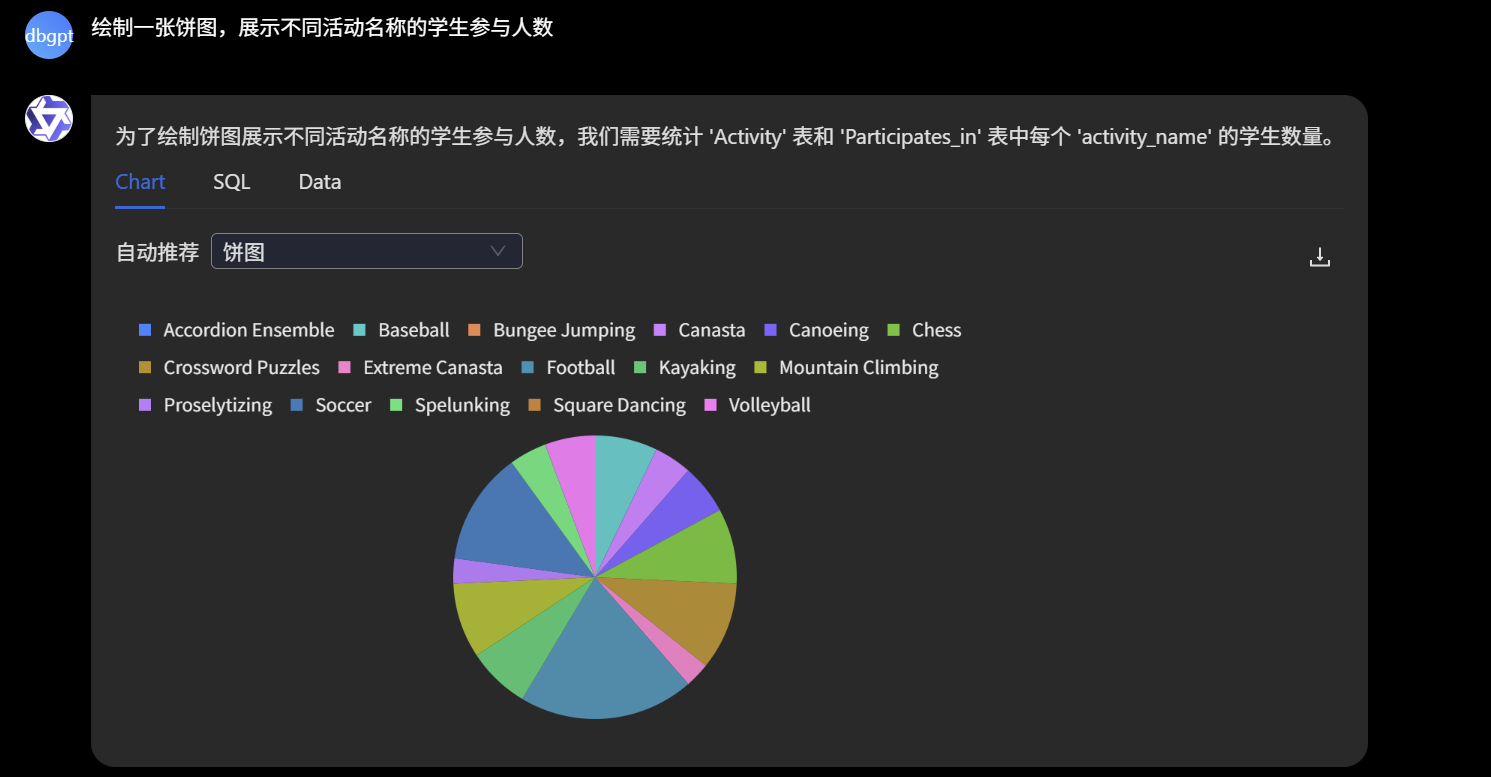
\includegraphics[width=11cm]{./images/27.问题5.png}
		\caption{问题5}
	\end{figure}
	
	\subsection{问题6}
	如何编写 SQL 语句来列出所有课程的名称,并按课程标题和学分排序?
	
	\begin{figure}[H]
		\centering
		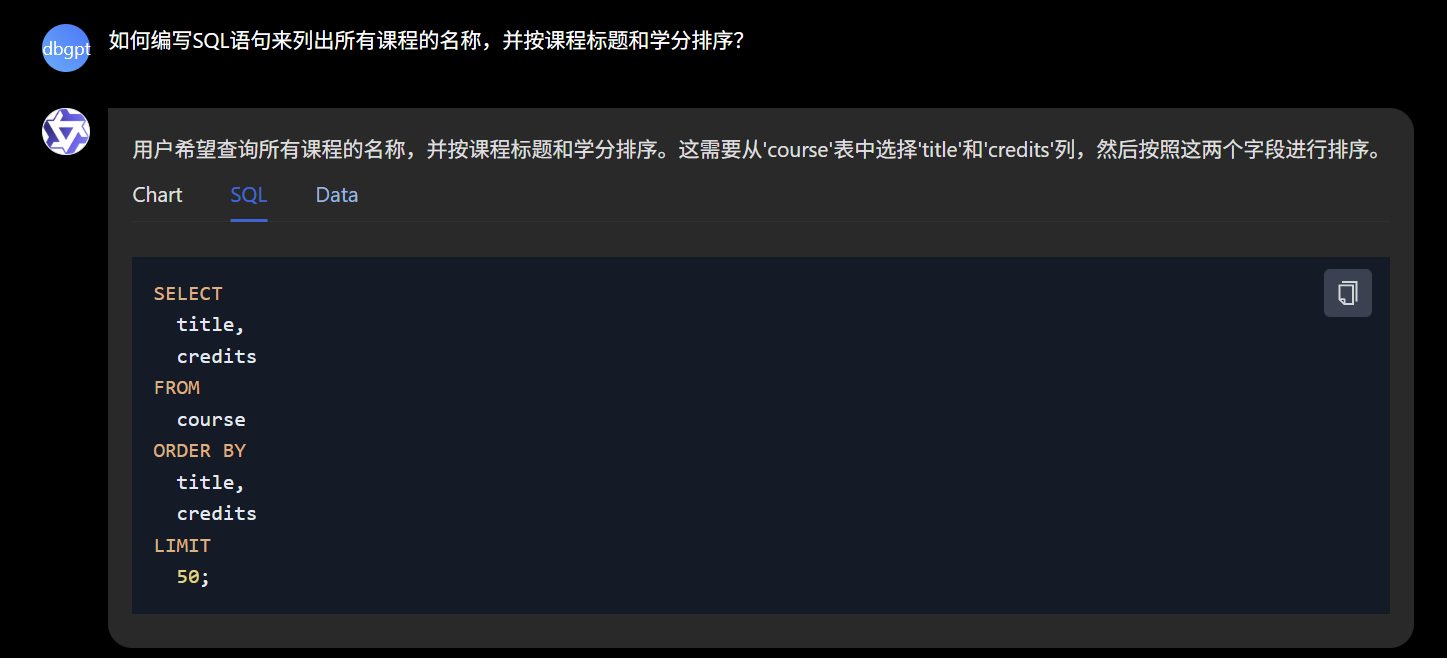
\includegraphics[width=11cm]{./images/28.问题6.png}
		\caption{问题6}
	\end{figure}
	
	\subsection{问题7}
	如何用 SQL 查询物理系提供的不同课程数量?
	
	\begin{figure}[H]
		\centering
		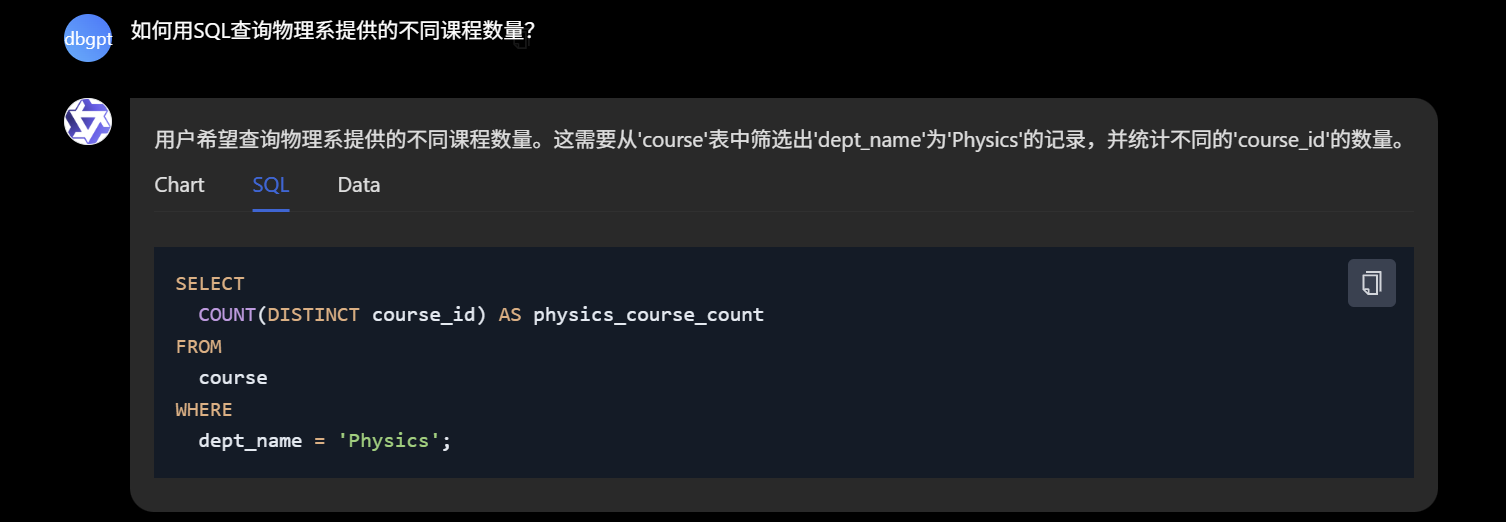
\includegraphics[width=11cm]{./images/29.问题7.png}
		\caption{问题7}
	\end{figure}
	
	返回结果10,符合预期
	
	\subsection{问题8}
	如何用统计图展示各部门的教师数量及其平均薪水?
	
	\begin{figure}[H]
		\centering
		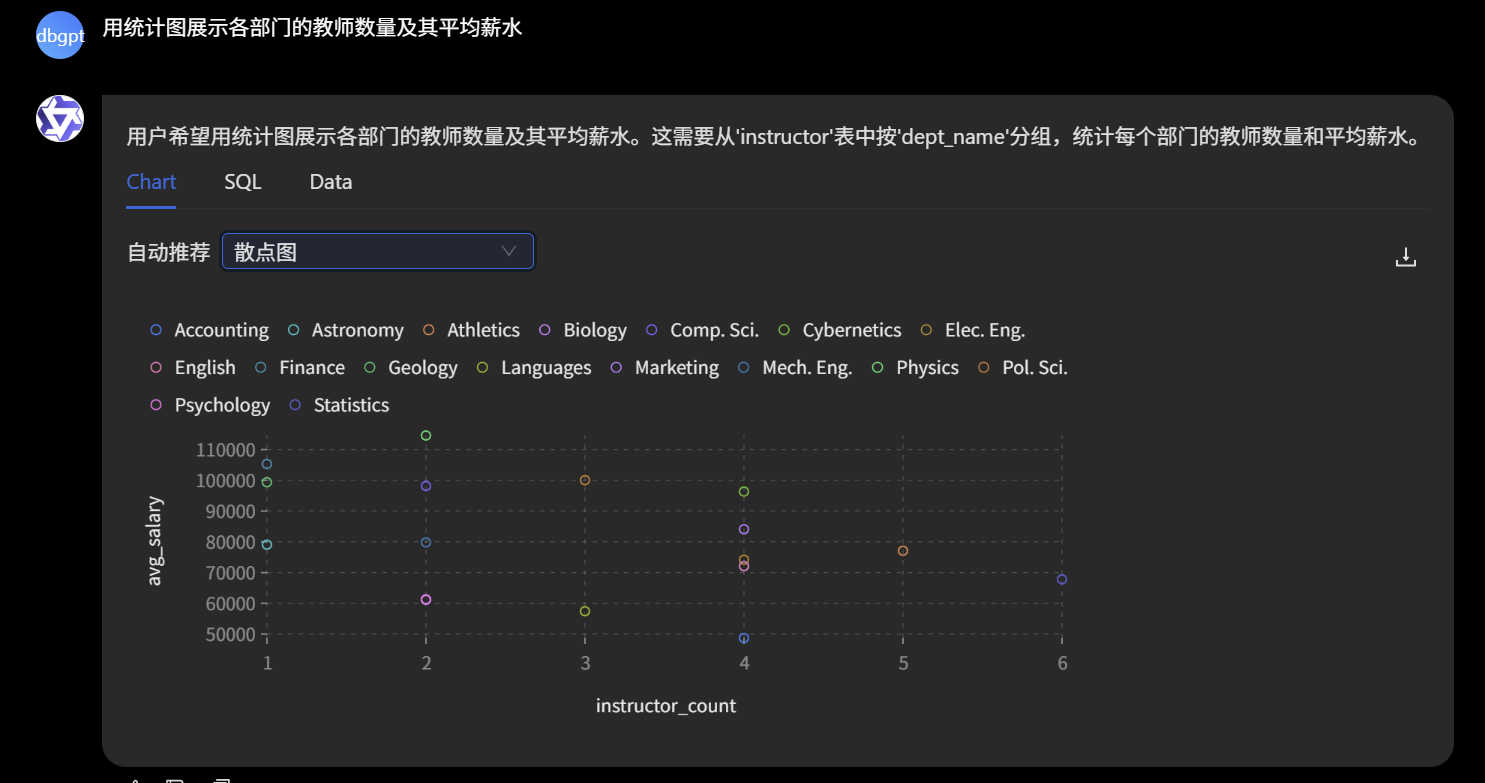
\includegraphics[width=11cm]{./images/30.问题8.png}
		\caption{问题8}
	\end{figure}
	
	这里我们发现,DB-GPT很智能的使用了散点图来清晰表示二维数据
	
	\subsection{问题9}
	如何用统计图展示各个教师授课课程的数量?
	
	DB-GPT给出了以下语句与结果:
	
	\begin{verbatim}
		SELECT
			ID,
			COUNT(DISTINCT course_id) AS course_count
		FROM
			teaches
		GROUP BY
			ID
		ORDER BY
			course_count DESC
		LIMIT
			50;
	\end{verbatim}
	
	\begin{figure}[H]
		\centering
		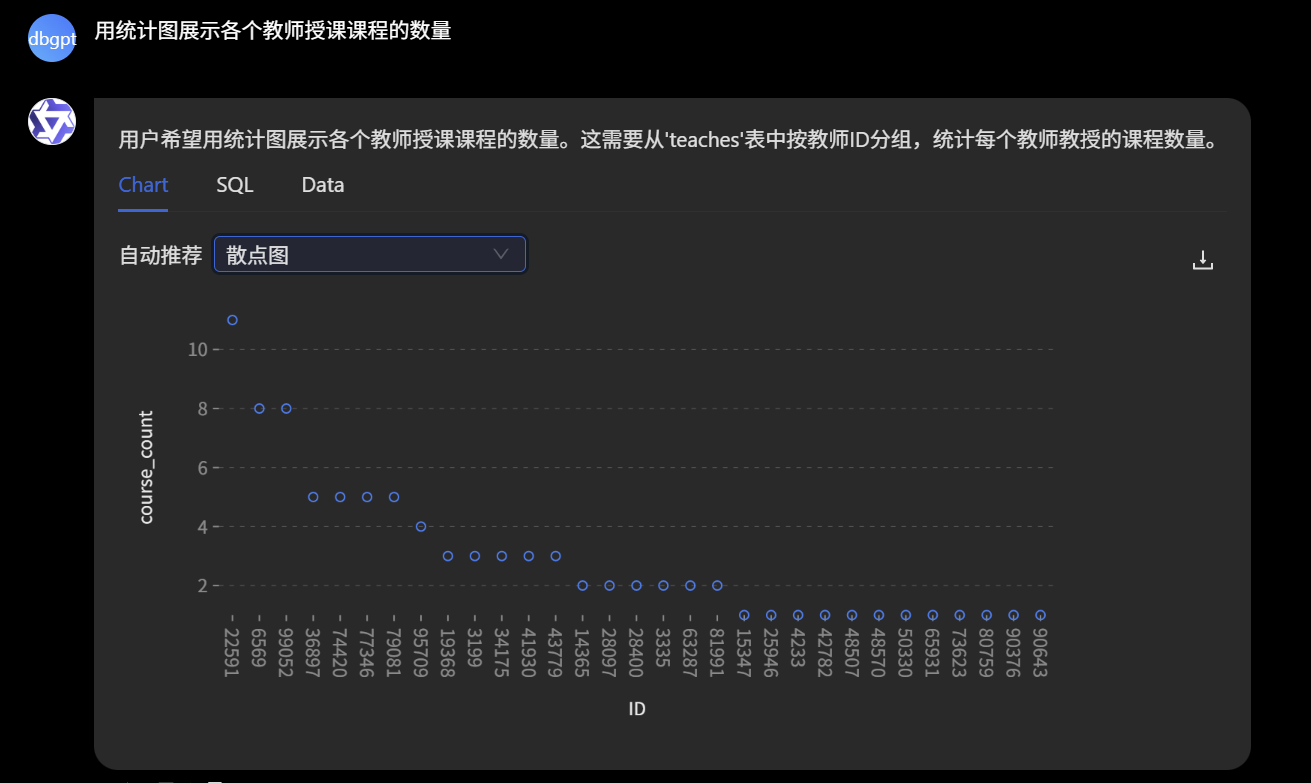
\includegraphics[width=11cm]{./images/31.问题9.png}
		\caption{问题9}
	\end{figure}
	
	\subsection{问题10}
	如何用饼图展示不同年级、不同学期的课程选修人数占总选修人数的比例?
	
	DB-GPT给出了以下语句与结果:
	
	\begin{verbatim}
		SELECT
			year || ' - ' || semester AS year_semester,
			COUNT(ID) AS student_count
		FROM
			takes
		GROUP BY
			year,
			semester
		LIMIT
			50;
	\end{verbatim}
	
	\begin{figure}[H]
		\centering
		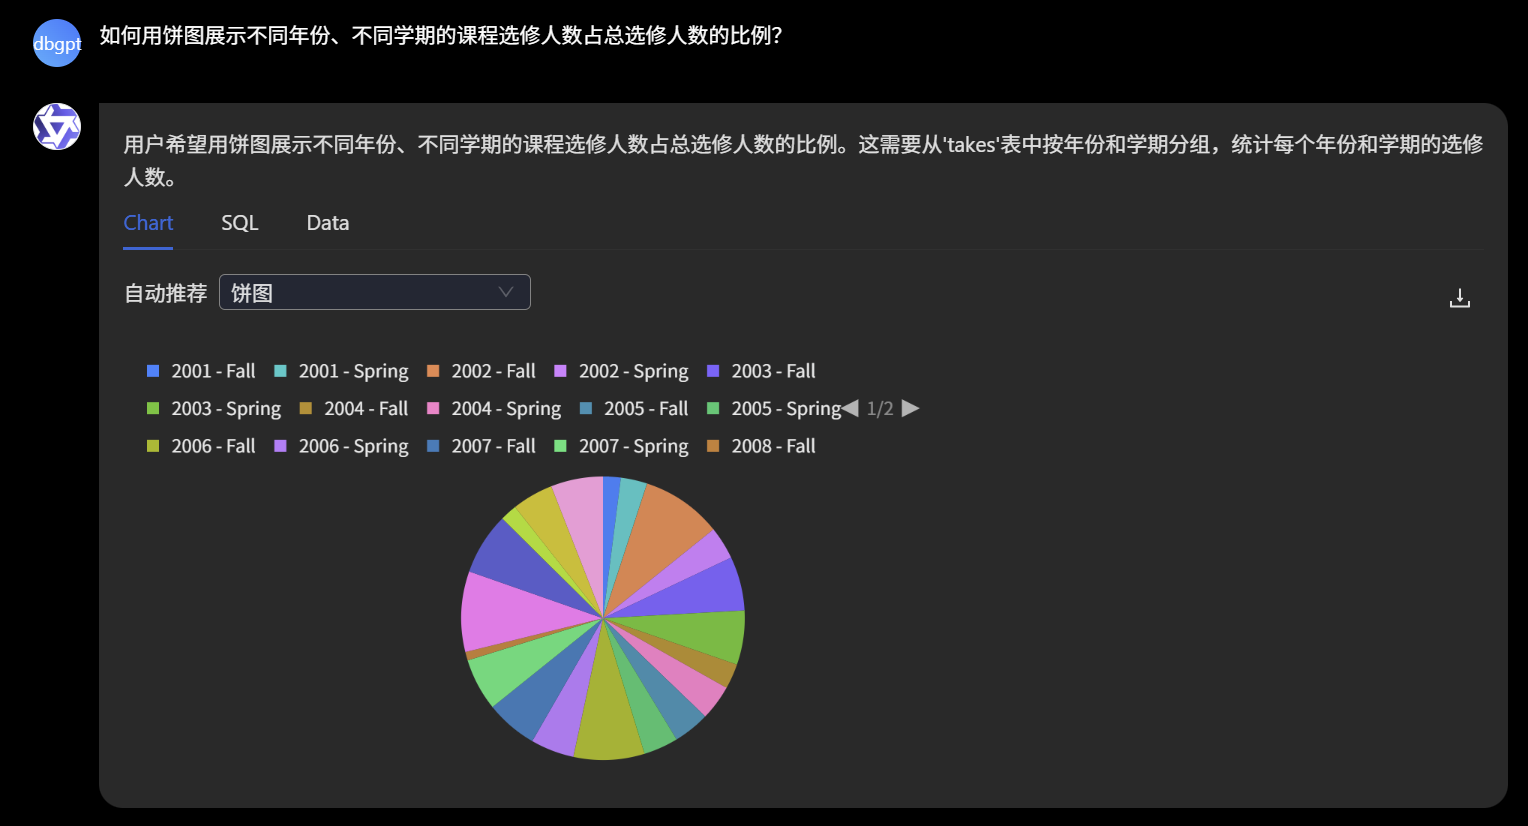
\includegraphics[width=11cm]{./images/32.问题10.png}
		\caption{问题10}
	\end{figure}
	
	\subsection{问题11}
	如何分析教师的授课负担?(例如,哪些教师在多个学期中教授了大量课程?)
	
	DB-GPT给出了以下语句与结果:
	
	\begin{verbatim}
		SELECT
			ID,
			semester,
			COUNT(DISTINCT course_id) AS course_count
		FROM
			teaches
		GROUP BY
			ID,
			semester
		ORDER BY
			course_count DESC
		LIMIT
			50;
	\end{verbatim}
	
	\begin{figure}[H]
		\centering
		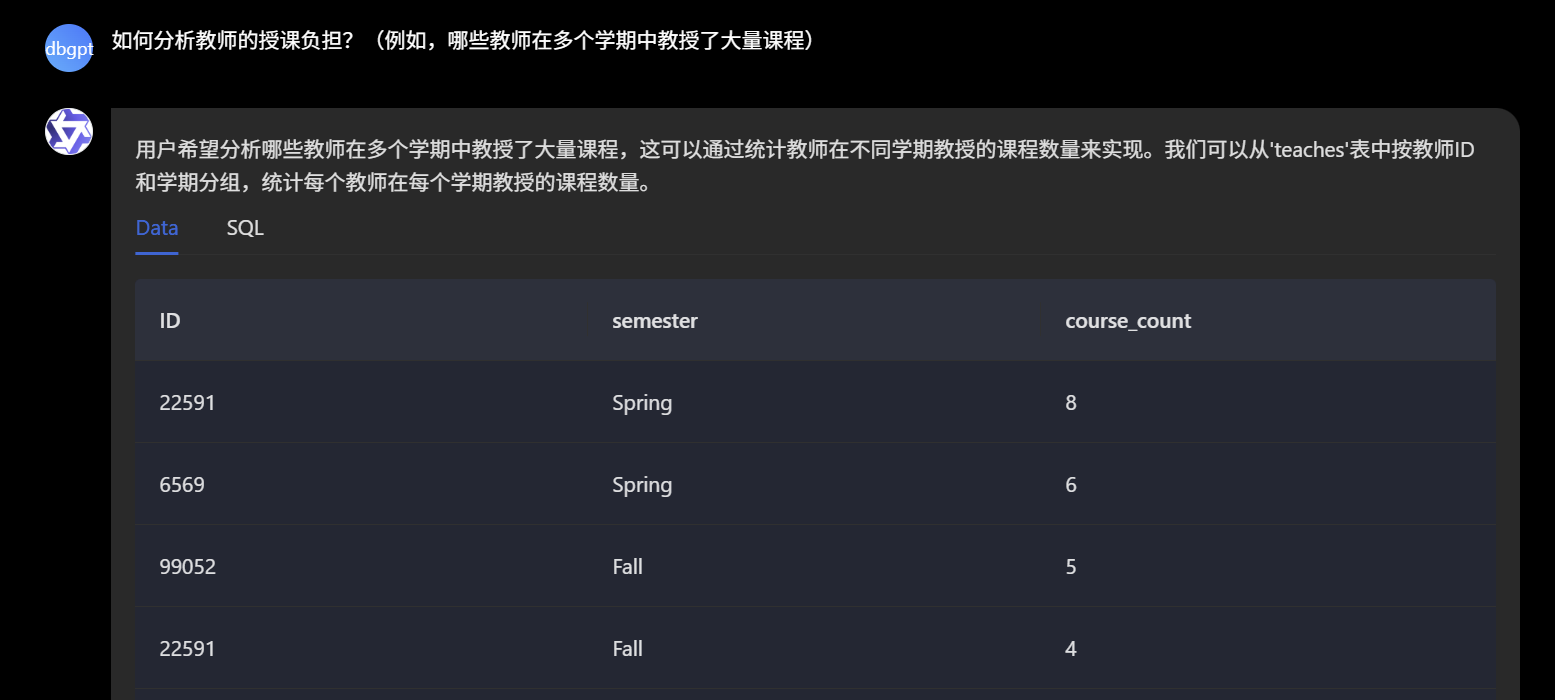
\includegraphics[width=11cm]{./images/33.问题11.png}
		\caption{问题11}
	\end{figure}
	
	\subsection{问题12}
	如何找出哪些课程是核心课程?(例如,这些课程连续开设了多年?)
	
	DB-GPT给出了以下语句与结果:
	
	\begin{verbatim}
		SELECT
			course_id,
			COUNT(DISTINCT year) AS years_taught
		FROM
			teaches
		GROUP BY
			course_id
		HAVING
			years_taught > 1
		ORDER BY
			years_taught DESC
		LIMIT
			50;
	\end{verbatim}
	
	\begin{figure}[H]
		\centering
		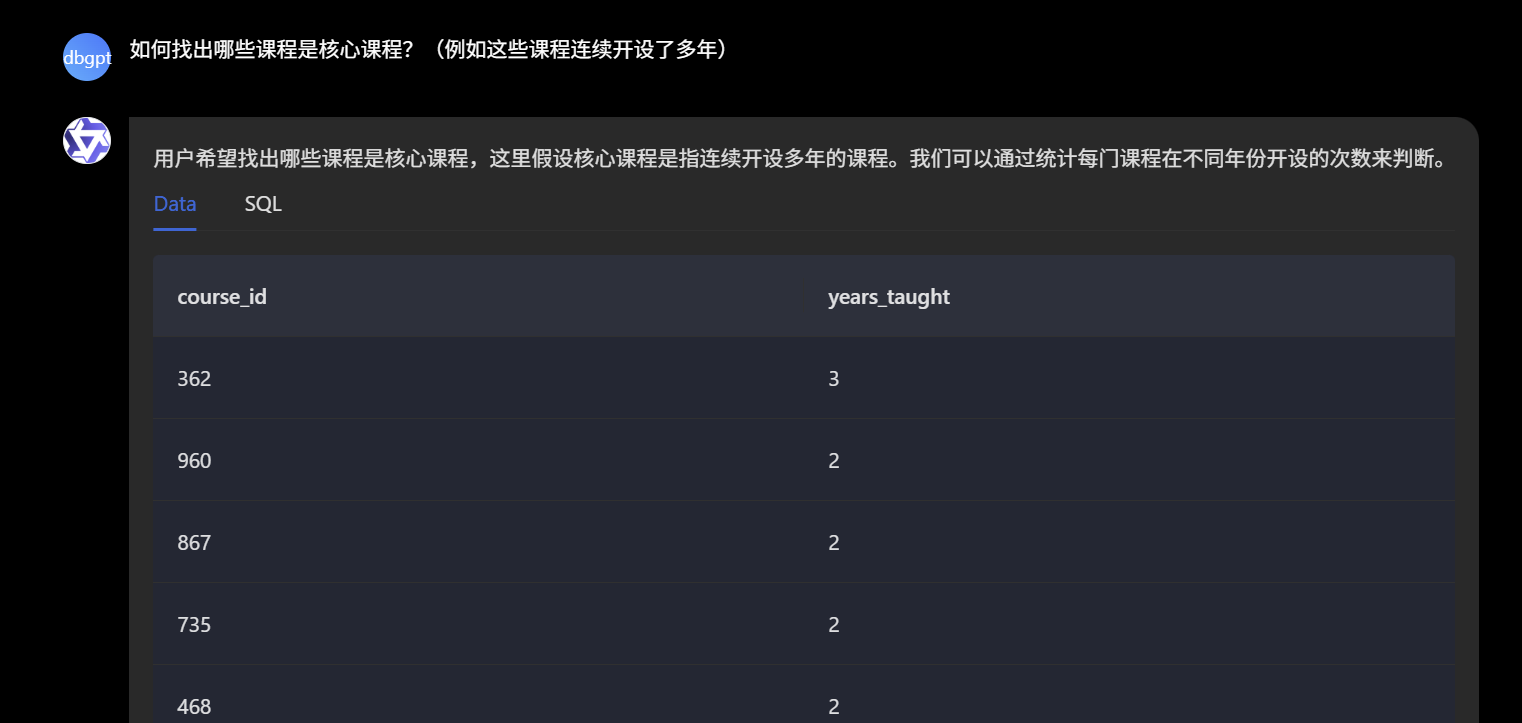
\includegraphics[width=11cm]{./images/34.问题12.png}
		\caption{问题12}
	\end{figure}
	
	\section{存在的问题及解决方案}
	
	本次实验中遇到了以下问题:
	
	\subsection{问题1}
	
	问题:git连接不成功,无法下载源代码
	
	解决:利用以下代码设置代理端口
	
	\begin{lstlisting}[language=bash, title=uv安装, tabsize=4]
		git config --global http.proxy socks5://127.0.0.1:26656
		git config --global https.proxy socks5://127.0.0.1:26656
	\end{lstlisting}
	
	\subsection{问题2}
	
	问题:遇到报错信息:error: Failed to fetch: `https://pypi.org/simple/charset-normalizer/`deng等
	
	解决:结果查询网上信息,得知是网络连接问题,重试即可
	
	\subsection{问题3}
	
	问题:配置文件修改不成功,网页会报错:invalid api
	
	解决:首先检查了api是否过期or额度用完,排除了这些情况之后,重新检查配置文件,通过查询官网的配置方法,将provider硬编码为:"proxy/openai",而非原本默认的"\${env:LLM\_MODEL\_PROVIDER:proxy/tongyi}"
	
	注释:其实也可以通过编辑环境变量来解决,但是此处采用了硬编码
	
	\subsection{问题4}
	
	问题:api直接放入文件会有安全隐患
	
	解决:配置环境变量,并使用echo \%DASHSCOPE\_API\_KEY\% 来检查是否配置完成,以及在配置文件中使用\$\{env:DASHSCOPE\_API\_KEY\}来调用环境变量
	
	\subsection{问题5}
	
	问题:原本的参考文档为旧版,很多内容与操作方法不一致
	
	解决:进入DB-GPT团队发布的官网,按照官网教程进行配置,最后顺利完成
	
	\section{实验小结}
	
	本次实验成功搭建了 DB-GPT 系统,完成了环境配置、功能测试和数据分析。实验验证了 DB-GPT 在自然语言处理和数据分析方面的强大能力,特别是在复杂查询、可视化输出和数据统计方面表现突出。实验中遇到了网络连接、性能瓶颈等问题,但通过优化硬件配置、改进算法逻辑和增强数据预处理能力,最终解决了这些挑战,确保了系统的稳定运行。
	
	未来,我们可以考虑如何优化 DB-GPT的问题,重点包括:提升模型性能,增加更多数据分析和可视化功能,增强用户体验,以及强化系统安全和可靠性。此外,计划引入多语言支持和自动部署能力,使其更具扩展性和易用性。通过持续改进,DB-GPT 将成为更高效、智能的数据驱动系统,为多领域用户提供强大支持。
	
\end{document}
